\documentclass{memoir}

\chapterstyle{hangnum}


\setcounter{secnumdepth}{2}


\usepackage{epigraph}
\usepackage{polyglossia}

\setmainlanguage[babelshorthands=true]{russian}    % Язык по-умолчанию русский с поддержкой приятных команд пакета babel
\setotherlanguage{english}                         % Дополнительный язык = английский (в американской вариации по-умолчанию)

%\setdefaultlanguage{russian}
%\setmainfont{CMU Serif}

%\setmonofont{Courier New}                          % моноширинный шрифт
%\newfontfamily\cyrillicfonttt{Courier New}         % моноширинный шрифт для кириллицы
%\defaultfontfeatures{Ligatures=TeX}                % стандартные лигатуры TeX, замены нескольких дефисов на тире и т. п. Настройки моноширинного шрифта должны идти до этой строки, чтобы при врезках кода программ в коде не применялись лигатуры и замены дефисов
%\setmainfont{Times New Roman}                      % Шрифт с засечками
%\newfontfamily\cyrillicfont{Times New Roman}       % Шрифт с засечками для кириллицы
%\setsansfont{Arial}                                % Шрифт без засечек
%\newfontfamily\cyrillicfontsf{Arial}               % Шрифт без засечек для кириллицы

\setmonofont{LiberationMono}[Scale=0.87]            % моноширинный шрифт
\newfontfamily\cyrillicfonttt{LiberationMono}[Scale=0.87]   % моноширинный шрифт для кириллицы
    
\defaultfontfeatures{Ligatures=TeX}                % стандартные лигатуры TeX, замены нескольких дефисов на тире и т. п. Настройки моноширинного шрифта должны идти до этой строки, чтобы при врезках кода программ в коде не применялись лигатуры и замены дефисов
\setmainfont{LiberationSerif}                      % Шрифт с засечками
%\setmainfont{CMU Serif}
\newfontfamily\cyrillicfont{LiberationSerif}       % Шрифт с засечками для кириллицы
\setsansfont{LiberationSans}                       % Шрифт без засечек
\newfontfamily\cyrillicfontsf{LiberationSans}      % Шрифт без засечек для кириллицы


\usepackage{amsthm}
\usepackage{url} 
\usepackage{hyperref} 


\usepackage[table]{xcolor}
%\let\newfloat\undefined
%\usepackage{floatrow}

% графика
\usepackage{graphicx}
\usepackage{tikz}                   % Продвинутый пакет векторной графики
\usepackage{pgfplots}
\pgfplotsset{compat=newest}
\usepackage{pgfplotstable}

\usepackage{wrapfig}

\usepackage{physics}
\usepackage{amsmath}
\usepackage{tikz}
\usepackage{mathdots}
\usepackage{yhmath}
\usepackage{cancel}
\usepackage{color}
\usepackage{siunitx}
\usepackage{array}
\usepackage{multirow}
\usepackage{amssymb}
\usepackage{gensymb}
\usepackage{tabularx}
\usepackage{booktabs}
\usetikzlibrary{fadings}
\usetikzlibrary{patterns}
\usetikzlibrary{shadows.blur}
\usetikzlibrary{shapes}




\begin{document}

\title{«Исследование скважин и пластов». Учебное пособие }
%\title{«Применение базовых алгоритмов анализа исследований нефтяных скважин»}
%\title{}

\maketitle

\tableofcontents{}
\chapter{Введение}

\section{Цели и задачи дисциплины}
Учебное пособие подготовлено в рамках курса "Исследования скважин и пластов", читаемого для студентов 4 курса РГУ нефти и газа (НИУ) имени И.М.Губкина и соответствует учебной программе курса по состоянию на 2020 год. 

Пособие описывает некоторые базовые подходы к построению и использованию математических моделей скважин и пластов, широко используемые при проведении и интерпретации исследований с использованием компьютеризированных алгоритмов. Рассматривается широкий диапазон исследований промысловых исследований - от технологических замеров ключевых параметров до внутрискважинных промысловых исследований и исследований пласта и призабойной зоны (во второй части). При этом акцент сделан именно на математических моделях и их реализациях в виде программных алгоритмов, что позволяет получить навыки построения моделей и интерпретации результатов исследований необходимые при широком использовании цифровых технологий в нефтедобычи. В работе широко используются открытые инструменты для проведения инженерных расчетов, что позволяет работать над решением задач на современном уровне без необходимости получения лицензий для коммерческих программ. 

Учебное пособие содержит набор задач, предназначенных для помощи в освоении дисциплины "Исследования скважин и пластов". Авторы уверены, что решение задач - лучший метод для изучения инженерных дисциплин. Поэтому в пособии сделан акцент именно на задачах. Теоретический материал приводится в минимальном виде, необходимом для решения задач. Для более подробного разбора теории приводятся ссылки на соответствующие материалы и статьи. Разобраны базовые примеры решения задач и приведены задачи для самостоятельной проработки в ходе семинаров. 

Пособие предназначено для студентов изучающих вопросы разработки и эксплуатации нефтяных и газовых месторождений, моделирование систем нефтедобычи, а также может быть полезным широкому кругу специалистов применяющих компьютерные математические модели нефтедобычи в практической деятельности. 

Учебное пособие является частью учебно методического комплекса для изучения дисциплины "Исследования скважин и пластов". Часть материалов комплекса доступна в сети интернет на общедоступных ресурсах. Это такие материалы как - программы и макросы для проведения инженерных расчетов, исходные данные для выполнения ряда заданий, видеоролики со вспомогательными материалами. Ссылки на ресурсы приводятся в пособии в состоянии актуальном на момент создания (предприняты все меры, чтобы обеспечить доступность ссылок на максимально длительный период, однако авторы не могут гарантировать работоспособность этих ссылок в длительной перспективе).




\section{Подход к изучению дисциплины Исследования скважин и пластов}
Курс "Исследования скважин и пластов" предназначен для того, чтобы дать студентам представление о современных подходах к проведению исследований на нефтяных месторождениях, а также о методах интерпретации их результатов. Рассматриваются различных виды исследований проводимых на скважинах введенных в эксплуатацию от технологических замеров и промысловых геофизических исследований до гидродинамических исследований.

Технологии проведения исследований и оборудование для их проведения с одной стороны достаточно хорошо описано в классической литературе и в интернет источниках, с другой стороны постоянно эволюционирует и меняется - появляются новые приборы и методы интерпретации, как правило использующие последние достижении техники и компьютерные технологии для интерпретации результатов. Остаются неизменными только физические принципы заложенные в основу исследований и методов их анализа. Понимая это авторы не гонятся за исчерпывающим описанием технологий и оборудования для проведения исследований. Вместо этого пособие описывает базовые принципы различных видов исследований выраженные в виде математических моделей. Причем рассматриваются компьютерные реализации этих моделей, которые могут быть использованы студентами и специалистами для обучения и для решения практических задач. Такие компьютерные модели лежат в основе большинства коммерческих программных комплексов, которые получили распространение в нефтяной промышленности, поэтому понимание основ их работы, сильных и слабых сторон, а также получение навыков построения компьютерных алгоритмов является залогом успешного и эффективного проведения исследования по глубокому убеждению авторов.

Большой объем материала и необходимость скорейшего создания учебного пособия заставили автором разбить пособие на две части. Часть 1 посвящена в большей степени исследованиям скважин - технологическим замерам (замеры дебита) и основам промысловых геофизических исследований (барометрия, термометрия и другие).  Часть 2 посвящена исследованию свойств пласта - гидродинамическим исследованиям скважин и построению простых моделей пласта и скважин - "прокси" моделям. При этом в этой части активно используют и модели скважин, разобранные в части 1.

В пособии рассматриваются принципы проведения и интерпретации распространенных видов исследований, которые лежат в основе многих расчетных методик. Понимание этих принципов и владение навыками проведения расчетов с использованием современных подходов позволит студенту решать широкий круг задач возникающих перед инженерами разработчиками на практике, а также облегчит самостоятельный разбор особенностей отдельных технологий. После разбора задач курса студенты смогут самостоятельно создать простые компьютерные алгоритмы для интерпретации базовых исследований скважин и пластов и при необходимости смогут развить их для обработки больших объемов данных по исследованиям и/или интерпретации нестандартных видов исследований. 

Из за широкого применения компьютерных алгоритмов в пособии читателю (и слушателю курсов) потребуется проявить навыки создания компьютерных программ. В простейшем варианте в виде создания сложных расчетных модулей в электронной таблице Excel. А в более "продвинутом" варианте в виде написания макросов и подпрограмм решающих определенные задачи. Это во многом отличает подход к изучению исследований скважин и пластов от других пособий и курсов известных авторам. Однако, опять же по глубокому убеждению авторов, эти навыки являются крайне полезными и востребованными в современной нефтедобыче, поэтому им уделяется особое внимание. Большинство задач можно решить без написания кода в явном виде (формулы в ячейках Excel по сути тоже являются компьютерным кодом, но здесь мы не имеем их в виду), однако умение создавать простые скрипты часто упрощает решение задач и позволяет применить решения для широкого спектра практически значимых проблем. Пособие не ставит целью научить какому то языку программирования. Подобных материалов много в интернете и ссылки на некоторые будут приведены. Пособие же сосредоточено больше на решении инженерных задач, для некоторых из которых применение элементов программирования может оказаться полезным. 





\chapter{Планирование и проектирование исследований}

Оценка экономической целесообразности проведения исследований. Ответ на вопрос - зачем нужны исследования. 
Будет про данные информацию и модели и описание зачем нужны модели и как правильно их использовать.
Соответственно большинство задач так или иначе посвящено использованию различных моделей. 
Тут будет про деревья решений среди прочего.

\section{Что мы будем понимать под исследованиями?}

\epigraph{Проблемы начинаются не тогда, когда имея в виду одно используют разные слова, а когда используя одни и теже слова имеют в виду разное.}{хорошо бы найти оригинал}

Проведение исследований неразрывно связано с понятиями -- данные, информация, знания. Эти термины всем знакомы, кажутся самодостаточными и очевидными. Их определения и различные трактовки можно легко найти в интернете, например на \url{https://ru.wikipedia.org/}.

\marginpar{
        \href{https://ru.wikipedia.org/wiki/информация}{Информация} 
        \newline
        
\includegraphics[scale=0.4]{pics/qr_wikipedia_information.png} 
        \newline
        \href{https://ru.wikipedia.org/wiki/данные}{Данные} 
        \newline
        
\includegraphics[scale=0.4]{pics/qr_wikipedia_data.png}
    }

Следствием распространённости этих понятий является многообразие их значений и интерпретаций в различных областях деятельности. Приведём здесь одну из интерпретаций, которой будем в дальнейшем придерживаться (\ref{ris:data_info_chart_1}. ). 

\begin{figure}[h!]
	\begin{center}
		

\tikzset{every picture/.style={line width=0.75pt}} %set default line width to 0.75pt        

\begin{tikzpicture}[x=0.75pt,y=0.75pt,yscale=-1,xscale=1]
%uncomment if require: \path (0,239); %set diagram left start at 0, and has height of 239

%Rounded Rect [id:dp8355723819738923] 
\draw [fill={rgb, 255:red, 184; green, 233; blue, 134 }  ,fill opacity=1 ]  (98,119.5) .. controls (98,115.08) and (101.58,111.5) .. (106,111.5) -- (202.97,111.5) .. controls (207.39,111.5) and (210.97,115.08) .. (210.97,119.5) -- (210.97,143.5) .. controls (210.97,147.92) and (207.39,151.5) .. (202.97,151.5) -- (106,151.5) .. controls (101.58,151.5) and (98,147.92) .. (98,143.5) -- cycle ;
%Rounded Rect [id:dp6680308810096447] 
\draw [fill={rgb, 255:red, 184; green, 233; blue, 134 }  ,fill opacity=1 ]  (270,119.5) .. controls (270,115.08) and (273.58,111.5) .. (278,111.5) -- (374.97,111.5) .. controls (379.39,111.5) and (382.97,115.08) .. (382.97,119.5) -- (382.97,143.5) .. controls (382.97,147.92) and (379.39,151.5) .. (374.97,151.5) -- (278,151.5) .. controls (273.58,151.5) and (270,147.92) .. (270,143.5) -- cycle ;
%Straight Lines [id:da6784338312341602] 
\draw    (211,131) -- (268,131) ;
\draw [shift={(268,131)}, rotate = 180] [color={rgb, 255:red, 0; green, 0; blue, 0 }  ][line width=0.75]    (10.93,-3.29) .. controls (6.95,-1.4) and (3.31,-0.3) .. (0,0) .. controls (3.31,0.3) and (6.95,1.4) .. (10.93,3.29)   ;

% Text Node
\draw (127,125) node [anchor=north west][inner sep=0.75pt]   [align=left] {Данные};
% Text Node
\draw (286,125) node [anchor=north west][inner sep=0.75pt]   [align=left] {Информация};

% Text Node
\draw (90,160) node [anchor=north west][inner sep=0.75pt]   [align=left] {То, что зафиксировано};
% Text Node
\draw (272,160) node [anchor=north west][inner sep=0.75pt]   [align=left] {То, что обработано};


\end{tikzpicture}

		\caption{Связь данных и информации}
		\label{ris:data_info_chart_1}
	\end{center}
\end{figure}

Под данными мы будем понимать совокупность сведений, зафиксированных на определенном носителе в форме пригодной для постоянного хранения обработки и интерпретации. Например замеры давления на приеме УЭЦН записанные в базу данных - это данные. Главное, что они записаны и к ним можно получить доступ при необходимости. 
Под информацией мы будем понимать результат преобразования и анализа данных направленный на практическую деятельность -- на принятие решений. Хотя информация должна обрести некоторую форму представления, то есть превратиться в данные, чтобы ей можно было обмениваться, информация есть в первую очередь интерпретация (смысл) такого представления. Информация всегда привязана к практической деятельности. Без применения, хотя бы потенциального, информация превращается в данные. 

Инженерная деятельность подразумевает постоянные действия для решения поставленных задач. Для нефтяного инжиниринга это эксплуатация месторождений углеводородов -- бурение скважине, проведение геолого-технических мероприятий. Действия или решения требуют необратимой траты ресурсов -- времени, материалов, денег. Из за ограниченности ресурсов возникает необходимость тщательного планирования действий -- принятия решений о необходимости действий. Мы часто будем использовать термин принятие решений и говорить о лице принимающем решение (ЛПР) для обозначения практической деятельности. Принятие решений -- это тот рубеж, который является целью исследований. Для принятия решений строятся модели, собираются данные и генерируется информация. 


Цепочку связи данных, информации и принятия решений можно отобразить схеме (рисунок  \ref{ris:data_info_decision_chart_1}). 

\begin{figure}[h!]
	\begin{center}
		

\tikzset{every picture/.style={line width=0.75pt}} %set default line width to 0.75pt        

\begin{tikzpicture}[x=0.75pt,y=0.75pt,yscale=-1,xscale=1]
%uncomment if require: \path (0,300); %set diagram left start at 0, and has height of 300

%Rounded Rect [id:dp2235462280724534] 
\draw  [fill={rgb, 255:red, 184; green, 233; blue, 134 }  ,fill opacity=1 ] (135.2,68) .. controls (135.2,63.58) and (138.78,60) .. (143.2,60) -- (227.97,60) .. controls (232.39,60) and (235.97,63.58) .. (235.97,68) -- (235.97,92) .. controls (235.97,96.42) and (232.39,100) .. (227.97,100) -- (143.2,100) .. controls (138.78,100) and (135.2,96.42) .. (135.2,92) -- cycle ;
%Rounded Rect [id:dp17536142021697776] 
\draw  [fill={rgb, 255:red, 184; green, 233; blue, 134 }  ,fill opacity=1 ] (293,68) .. controls (293,63.58) and (296.58,60) .. (301,60) -- (388.97,60) .. controls (393.39,60) and (396.97,63.58) .. (396.97,68) -- (396.97,92) .. controls (396.97,96.42) and (393.39,100) .. (388.97,100) -- (301,100) .. controls (296.58,100) and (293,96.42) .. (293,92) -- cycle ;
%Straight Lines [id:da11139667469680425] 
\draw    (264.92,45.28) -- (264.92,78) ;
\draw [shift={(264.92,80)}, rotate = 270] [color={rgb, 255:red, 0; green, 0; blue, 0 }  ][line width=0.75]    (10.93,-3.29) .. controls (6.95,-1.4) and (3.31,-0.3) .. (0,0) .. controls (3.31,0.3) and (6.95,1.4) .. (10.93,3.29)   ;
%Rounded Rect [id:dp3985813066419075] 
\draw  [fill={rgb, 255:red, 184; green, 233; blue, 134 }  ,fill opacity=1 ] (457,68) .. controls (457,63.58) and (460.58,60) .. (465,60) -- (594.52,60) .. controls (598.94,60) and (602.52,63.58) .. (602.52,68) -- (602.52,92) .. controls (602.52,96.42) and (598.94,100) .. (594.52,100) -- (465,100) .. controls (460.58,100) and (457,96.42) .. (457,92) -- cycle ;
%Straight Lines [id:da985211792743889] 
\draw    (397.4,80) -- (455.11,80) ;
\draw [shift={(457.11,80)}, rotate = 180] [color={rgb, 255:red, 0; green, 0; blue, 0 }  ][line width=0.75]    (10.93,-3.29) .. controls (6.95,-1.4) and (3.31,-0.3) .. (0,0) .. controls (3.31,0.3) and (6.95,1.4) .. (10.93,3.29)   ;
%Rounded Rect [id:dp8115508928060304] 
\draw  [fill={rgb, 255:red, 245; green, 166; blue, 35 }  ,fill opacity=1 ] (210.11,13.28) .. controls (210.11,8.86) and (213.69,5.28) .. (218.11,5.28) -- (311.73,5.28) .. controls (316.15,5.28) and (319.73,8.86) .. (319.73,13.28) -- (319.73,37.28) .. controls (319.73,41.7) and (316.15,45.28) .. (311.73,45.28) -- (218.11,45.28) .. controls (213.69,45.28) and (210.11,41.7) .. (210.11,37.28) -- cycle ;
%Straight Lines [id:da5256470314414583] 
\draw    (235.97,80) -- (290.71,80) ;
\draw [shift={(292.71,80)}, rotate = 180] [color={rgb, 255:red, 0; green, 0; blue, 0 }  ][line width=0.75]    (10.93,-3.29) .. controls (6.95,-1.4) and (3.31,-0.3) .. (0,0) .. controls (3.31,0.3) and (6.95,1.4) .. (10.93,3.29)   ;

% Text Node
\draw (186.09,79.95) node   [align=left] {Данные};
% Text Node
\draw (343.91,79.95) node   [align=left] {Информация};
% Text Node
\draw (529.76,80) node   [align=left] {Принятие решений};
% Text Node
\draw (264.81,24.62) node   [align=left] {Исследование};


\end{tikzpicture}
		\caption{Связь данных, информации и принятия решений}
		\label{ris:data_info_decision_chart_1}
	\end{center}
\end{figure}

Схема показывает, что информация напрямую связана с принятием решений. Если мы не понимаем зачем необходима информация -- на принятие какого решения она работает, то она может оказаться бессмысленной. В приведенной схеме процесс преобразования данных в информацию можно назвать исследованием. 
Цель исследования -- обеспечить процесс принятия решений информаций. И аналогично информации -- исследование имеет смысл только если направлено на принятие решений. 
\marginpar{
	\href{https://ru.wikipedia.org/wiki/исследование}{Исследование} 
	
\includegraphics[scale=0.4]{pics/qr_wikipedia_investigation.png} } 
Схему можно еще дополнить добавив в нее инструмент для преобразования данных в информацию и принятия решений на основе информации -- модель. Чаще всего имеются в виду математические модели в виде компьютерных алгоритмов. Именно их мы будет использовать, но на их месте могут быть и другие модели (например интуиция лица принимающего решения или его опыт). 

\begin{figure}[h!]
	\begin{center}
		

\tikzset{every picture/.style={line width=0.75pt}} %set default line width to 0.75pt        

\begin{tikzpicture}[x=0.75pt,y=0.75pt,yscale=-1,xscale=1]
%uncomment if require: \path (0,300); %set diagram left start at 0, and has height of 300

%Rounded Rect [id:dp597190226460943] 
\draw   (113.2,151) .. controls (113.2,146.58) and (116.78,143) .. (121.2,143) -- (208.97,143) .. controls (213.39,143) and (216.97,146.58) .. (216.97,151) -- (216.97,175) .. controls (216.97,179.42) and (213.39,183) .. (208.97,183) -- (121.2,183) .. controls (116.78,183) and (113.2,179.42) .. (113.2,175) -- cycle ;
%Rounded Rect [id:dp3409304527040422] 
\draw   (274,151) .. controls (274,146.58) and (277.58,143) .. (282,143) -- (378.97,143) .. controls (383.39,143) and (386.97,146.58) .. (386.97,151) -- (386.97,175) .. controls (386.97,179.42) and (383.39,183) .. (378.97,183) -- (282,183) .. controls (277.58,183) and (274,179.42) .. (274,175) -- cycle ;
%Straight Lines [id:da9955922595564108] 
\draw    (216,163) -- (273.2,163) ;
\draw [shift={(275.2,163)}, rotate = 180] [color={rgb, 255:red, 0; green, 0; blue, 0 }  ][line width=0.75]    (10.93,-3.29) .. controls (6.95,-1.4) and (3.31,-0.3) .. (0,0) .. controls (3.31,0.3) and (6.95,1.4) .. (10.93,3.29)   ;
%Rounded Rect [id:dp45297167935805027] 
\draw   (451,151) .. controls (451,146.58) and (454.58,143) .. (459,143) -- (574.2,143) .. controls (578.62,143) and (582.2,146.58) .. (582.2,151) -- (582.2,175) .. controls (582.2,179.42) and (578.62,183) .. (574.2,183) -- (459,183) .. controls (454.58,183) and (451,179.42) .. (451,175) -- cycle ;
%Straight Lines [id:da11147374736012572] 
\draw    (388.2,161.94) -- (447.2,162) ;
\draw [shift={(449.2,162)}, rotate = 180.06] [color={rgb, 255:red, 0; green, 0; blue, 0 }  ][line width=0.75]    (10.93,-3.29) .. controls (6.95,-1.4) and (3.31,-0.3) .. (0,0) .. controls (3.31,0.3) and (6.95,1.4) .. (10.93,3.29)   ;
%Rounded Rect [id:dp851243700176072] 
\draw   (211.2,209) .. controls (211.2,204.58) and (214.78,201) .. (219.2,201) -- (442.2,201) .. controls (446.62,201) and (450.2,204.58) .. (450.2,209) -- (450.2,233) .. controls (450.2,237.42) and (446.62,241) .. (442.2,241) -- (219.2,241) .. controls (214.78,241) and (211.2,237.42) .. (211.2,233) -- cycle ;
%Straight Lines [id:da1477687213170571] 
\draw    (245,200.5) -- (245.57,165) ;
\draw [shift={(245.6,163)}, rotate = 450.92] [color={rgb, 255:red, 0; green, 0; blue, 0 }  ][line width=0.75]    (10.93,-3.29) .. controls (6.95,-1.4) and (3.31,-0.3) .. (0,0) .. controls (3.31,0.3) and (6.95,1.4) .. (10.93,3.29)   ;
%Straight Lines [id:da9162736044666429] 
\draw    (419,199.5) -- (419.57,164) ;
\draw [shift={(419.6,162)}, rotate = 450.92] [color={rgb, 255:red, 0; green, 0; blue, 0 }  ][line width=0.75]    (10.93,-3.29) .. controls (6.95,-1.4) and (3.31,-0.3) .. (0,0) .. controls (3.31,0.3) and (6.95,1.4) .. (10.93,3.29)   ;

% Text Node
\draw (137,153.5) node [anchor=north west][inner sep=0.75pt]   [align=left] {Данные};
% Text Node
\draw (285,154.5) node [anchor=north west][inner sep=0.75pt]   [align=left] {Информация};
% Text Node
\draw (460,153.5) node [anchor=north west][inner sep=0.75pt]   [align=left] {Принятие решений};
% Text Node
\draw (304,212.5) node [anchor=north west][inner sep=0.75pt]   [align=left] {Модель};


\end{tikzpicture}

		\caption{Связь данных, информации, принятия решений и моделирования}
		\label{ris:data_model_chart_1}
	\end{center}
\end{figure}

Именно такого подхода мы будем придерживаться в курсе и данном пособии. Такое определение, хотя и несколько отличается от классических, обладает рядом преимуществ. Например позволяет оценить когда надо проводить исследования и сколько ресурсов на них можно потратить или увидеть как можно некоторые виды деятельности, изначально не направленные на получение информации, рассматривать в качестве исследований и извлечь из них дополнительную ценность.
 \marginpar{
 	\href{https://www.gazprom-neft.ru/press-center/sibneft-online/archive/2018-may/1589542/} {Газпром нефть. Цифровизация — это фундаментальный тренд}.
 	
\includegraphics[scale=0.4]{pics/qr_digitalization.png} }  
Например с развитием информационных технологий в нефтедобычи все больше информации о нормальной эксплуатации скважины накапливается в базах данных добывающих компаний. Эти данные содержат информацию о том как работают скважины и месторождения. Если их рассмотреть как исследования -- их можно преобразовать в информацию и использовать ее для принятия решений, например о проведении ГТМ, без необходимости траты ресурсов на проведение классических исследований. Это направление сейчас активно развивается в нефтяной промышленности под знамёнами цифровизации и в рамках курса будет неоднократно обсуждаться.

Подумайте как можно на приведённые схемы добавить категорию - знание? Как могут быть связаны исследования и знания?

\section{Ожидаемая ценность в условиях неопределённости -- EMV}

Исследования почти всегда идут рядом с неопределённостями различного вида. Неопределённости могут быть связаны с параметрами изучаемых объектов. Например планируя пробурить скважину, мы хотели бы знать ее дебит. Мы знаем, что дебит будет зависеть от проницаемости пласта, но проницаемость мы не знаем -- мы находимся в ситуации неопределённости. 

Мы  можем описать неопределённость проницаемости задав вероятные исходы для значения проницаемости. Пусть мы ожидаем, что величина проницаемости задаётся следующим распределением:

\begin{itemize}
	\item $k_1 = 10$ мД с вероятностью $P_1 = 0.2$; 
	\item $k_2 = 20$ мД с вероятностью $P_2 = 0.6$; 
	\item $k_3 = 30$ мД с вероятностью $P_3 = 0.2$. 
\end{itemize}

Если мы рассмотрим задачу строительства новой скважины на месторождении с заданными параметрами, тогда дебиты скважины могут оценены из выражения

\begin{equation}
	Q = \frac{kh}{18.41 \mu B} \frac{\Delta P}{  \left( ln\dfrac{r_e}{r_w} + S\right) }
	\label{eq:eq_q}
\end{equation}

$Q$ -- дебит скважины ожидаемый;

$k$ -- проницаемость пласта, мД;

$h$ -- мощность пласта, м;

$\mu$ -- вязкость нефти, сП;

$B$ -- объемный коэффициент нефти, м$^3$/м$^3$

$\Delta P$ -- депрессия на пласт, атм;

$r_e$ -- радиус контура дренирования скважины, м;

$r_w$ -- радиус скважины, м;

$S$ -- скин-фактор скважины, м;


а доход от эксплуатации скважины в течении периода времени  $\Delta T$

\begin{equation}
	MV = Q \cdot  \Delta T \cdot  Price_{oil} - Price_{well}
	\label{eq:eq_MV}
\end{equation}

где 

$MV$ -- доход от эксплуатации (monetary value);

$Q$ -- дебит скважины ожидаемый;
 
$\Delta T$ -- период времени за который проходит оценка;

$Price_{oil}$ -- стоимость единицы добычи нефти.

$Price_{well}$ -- стоимость строительства скважины

Тогда подставляя \eqref{eq:eq_q} в \eqref{eq:eq_MV} получим 

\begin{equation}
	MV = \alpha k - \beta
	\label{eq:eq_MV_2}
\end{equation}

где 

$$\alpha =  \Delta T \cdot  Price \cdot \frac{h}{18.41 \mu B} \frac{\Delta P}{  \left( ln\dfrac{r_e}{r_w} + S\right)}
$$ 

$$
\beta = Price_{well}
$$

параметры, который мы предполагаем постоянными в рамках данной модели. 

Тогда ожидаемую доходность с учётом неопределённости можно получить как математическое ожидание доходности с учётом заданного распределения. 

\begin{equation}
	EMV = \sum_{i} MV \cdot P_i 
\end{equation}

Величину ожидаемой доходности можно представить в виде графической диаграммы, приведённой на рисунке \ref{ris:chance_node}.

Чтобы более наглядно представить последующие рассуждения, приведём численный пример.Предположим, что величина $\alpha = 1$, $\beta = 15$. Размерности величин не указываем, но понимаем, что это некоторый финансовый показатель.  

Тогда получим для случая строительства скважины с приведёнными выше априорными показателями 

\begin{multline}
	EMV = \sum_{i} (\alpha k_i - \beta ) P_i = \\
	= (1 \cdot 10 - 15) \cdot 0.2 + (1 \cdot 20 - 15)\cdot 0.6 + (1 \cdot 30 - 15)\cdot 0.2 = 5
\end{multline}

Для заданный условий получаем $EMV =5 > 0$, что можно интерпретировать, что в среднем бурение скважины в этих условиях будет рентабельно.


\begin{figure}[h!]
	\tikzset{every picture/.style={line width=0.75pt}} %set default line width to 0.75pt        
	\centering
	\begin{tikzpicture}[x=0.75pt,y=0.75pt,yscale=-1,xscale=1]
		%uncomment if require: \path (0,300); %set diagram left start at 0, and has height of 300
		
		%Straight Lines [id:da9914598188026227] 
		\draw    (125,128) -- (237.4,41) ;
		%Straight Lines [id:da8494600211227674] 
		\draw    (125,128) -- (237.4,215.45) ;
		%Straight Lines [id:da3455826146339449] 
		\draw    (125,128) -- (237.4,128) ;
		%Shape: Circle [id:dp4694470217534936] 
		\draw  [fill={rgb, 255:red, 248; green, 231; blue, 28 }  ,fill opacity=1 ] (103.95,128) .. controls (103.95,116.37) and (113.37,106.95) .. (125,106.95) .. controls (136.63,106.95) and (146.05,116.37) .. (146.05,128) .. controls (146.05,139.63) and (136.63,149.05) .. (125,149.05) .. controls (113.37,149.05) and (103.95,139.63) .. (103.95,128) -- cycle ;
		%Shape: Triangle [id:dp6993619331790251] 
		\draw  [fill={rgb, 255:red, 184; green, 233; blue, 134 }  ,fill opacity=1 ] (237.4,41) -- (267.48,21.01) -- (267.39,61.11) -- cycle ;
		%Shape: Triangle [id:dp5948591148628843] 
		\draw  [fill={rgb, 255:red, 184; green, 233; blue, 134 }  ,fill opacity=1 ] (237.4,127.97) -- (267.48,107.98) -- (267.39,148.08) -- cycle ;
		%Shape: Triangle [id:dp600205010959115] 
		\draw  [fill={rgb, 255:red, 184; green, 233; blue, 134 }  ,fill opacity=1 ] (237.4,215.42) -- (267.48,195.43) -- (267.39,235.53) -- cycle ;
		
		% Text Node
		\draw (174,50) node [anchor=north west][inner sep=0.75pt]    {$p_{1}, k_1$};
		% Text Node
		\draw (174,106) node [anchor=north west][inner sep=0.75pt]    {$p_{2}, k_2$};
		% Text Node
		\draw (174,146) node [anchor=north west][inner sep=0.75pt]    {$p_{3}, k_3$};
		% Text Node
		\draw (277,19) node [anchor=north west][inner sep=0.75pt]    {$MV_{1}$};
		% Text Node
		\draw (277,106) node [anchor=north west][inner sep=0.75pt]    {$MV_{2}$};
		% Text Node
		\draw (277,193) node [anchor=north west][inner sep=0.75pt]    {$MV_{3}$};
		% Text Node
		\draw (92,162) node [anchor=north west][inner sep=0.75pt]    {$\sum p_{i} MV_{i}$};
	\end{tikzpicture}
	\label{ris:chance_node}
	\caption{Графическое представление для вычисления ожидаемой доходности EMV}
\end{figure}

Здесь мы, следуя соглашения для отрисовки деревьев решений, в виде круга обозначили вероятностный узел -  выходами из которого являются ветви дерева, представляющие возможные дискретные исходы задаваемым природой или постановкой задачи - исходы на которые мы не можем повлиять. Конечные исходы обозначаем треугольниками. Каждая ветвь выходящая из вероятностного узла характеризуется вероятностью и значением проницаемости (для нашей задачи), каждый исход описывается величиной доходности при заданной вероятности. 

%надо доделать тут

\section{Ценность информации полученной в ходе исследований -- VOI}

Хорошим вопросом касательно любых исследований и даже шире -- любых расчётов и инженерных моделей -- является вопрос -- зачем всем этим надо заниматься? Задав этот вопрос, можно услышать много ответов. Часто говорят -- чтобы лучше изучить месторождение, чтобы определить параметры месторождения или скважины, чтобы рассчитать оптимальный режим работы скважины. Такие ответы верны, но в тоже время слишком расплывчаты. Попробуйте поставить себя на место главного инженера добывающего предприятия и оценить -- выделили бы вы ценные ресурсы молодому специалисту который предлагает лучше изучить какую-то скважину? 

Лица принимающие решения (главный инженер добывающего предприятия -- хорошая модель ЛПР для нашего курса) любят более конкретные обоснования как правило. Лучше всего экономические.

Один из ответов на вопрос -- "Зачем проводить исследования?" можно получить с использованием понятия ценности информации (Value of Information). 

\marginpar{
        \href{https://ru.wikipedia.org/wiki/ценность_информации}{Ценность информации} 
        
\includegraphics[scale=0.4]{pics/qr_wikipedia_VOI.png} 
        }

Согласно упрощённой версии этого подхода можно допустить, что ценность информации полученного в ходе исследования равна разнице в эффективности принятого решения с учётом этой информации и без ее учёта. 

\begin{equation}
	\label{eq:VOI}
	VOI = EMV_{inf}-EMV_{0} 
\end{equation}

Здесь $VOI$ - ценность информации, $EMV_{inf}$ - ожидаемая ценность принятого решения с учетом информации (estimated monetary value), $EMV_{0}$ - ожидаемая ценность принятого решения без учёта информации.

То есть ценность исследования, а следовательно и целесообразность его проведения (затрат ресурсов на его проведение) целиком зависит от эффективности принятых решений. 

Предположим, что для приведённых выше условий по априорному распределению проницаемости в пласте имеется возможность провести ГДИС и уточнить величины проницаемости. 

Например мы ожидаем, что после исследования мы сможем снизить неопределённость в проницаемости и тем самым уточнить дебит скважины после запуска.  

Предположим, что можно выделить два исхода распределения вероятности после проведения теста

Первый с вероятностью $p_1 = 0.5$

\begin{itemize}
	\item $k_1 = 10$ мД с вероятность $P_1 = 0.2$; 
	\item $k_2 = 15$ мД с вероятность $P_2 = 0.6$; 
	\item $k_3 = 20$ мД с вероятность $P_3 = 0.2$. 
\end{itemize}

Второй с вероятностью $p_1 = 0.5$

\begin{itemize}
	\item $k_1 = 20$ мД с вероятность $P_1 = 0.2$; 
	\item $k_2 = 25$ мД с вероятность $P_2 = 0.6$; 
	\item $k_3 = 30$ мД с вероятность $P_3 = 0.2$. 
\end{itemize}

\begin{figure}[h!]
	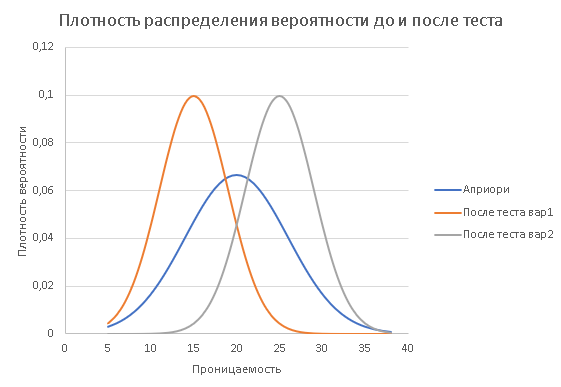
\includegraphics[width= 15cm]{pics_2/norm_distribution_ex1.png} 
	\label{fig:sample2}
	\caption{Иллюстрация к уточнению проницаемости в ходе исследований}
\end{figure}

Такой подход является явным упрощением. По приведённым ссылкам можно найти и другие подходы, где в частности предлагается учесть и менее явные последствия. Но его преимущество как раз в простоте. Он позволяет количественно оценить эффект от проведения исследований, соотнести его с затратами на проведение исследований и построить критерий принятия решений, который уже можно далее обсуждать и улучшать. 


Существует много подходов к построению критерия принятия решений о необходимости проведения исследований [ссылка на making good decisions]. Мы рассмотрим один из них, широко применяемый в различных областях деятельности, особенной в экономике и компьютерных науках - метод построения деревьев решений. \cite{AL_appl_patt_2007}

\section{Деревья решений для планирования исследований}

% translation from https://github.com/SilverDecisions/SilverDecisions/wiki/1.-Decision-tree-model
Последовательность и неопределенность присущи практическому принятию решений. Первое означает, что лица, принимающие решения, должны рассматривать многоступенчатые стратегии, охватывающие несколько действий, следующих друг за другом, а не только одно действие. Вторая означает, что отдача, получаемая лицами, принимающими решения, зависит не только от действий, но и от внешних событий ( состояний мира), которые часто могут быть восприняты как случайные. Действия и реакции обычно переплетаются, что еще больше усложняет картину. Деревья решений используются в качестве модели, помогающей обнаружить, понять и передать структуру таких проблем, связанных с принятием решений.

Ниже представлено простое дерево решений, созданное с помощью программы SilverDecisions (файл SilverDecisions, содержащий это дерево, можно запустить \href{http://silverdecisions.pl/SilverDecisions.html?LOAD_SD_TREE_JSON=https://raw.githubusercontent.com/gubkin-rienm/isp/master/data/decision_tree/simple_invest_decision.json}{здесь}).
\marginpar{
        ссылку там есть - надо сделать QR на нее
        }
%\urldef{\myurl}{http://silverdecisions.pl/SilverDecisions.html?LOAD_SD_TREE_JSON=https://raw.githubusercontent.com/gubkin-rienm/isp/master/data/decision_tree/simple_invest_decision.json}

\begin{figure}[h!]
	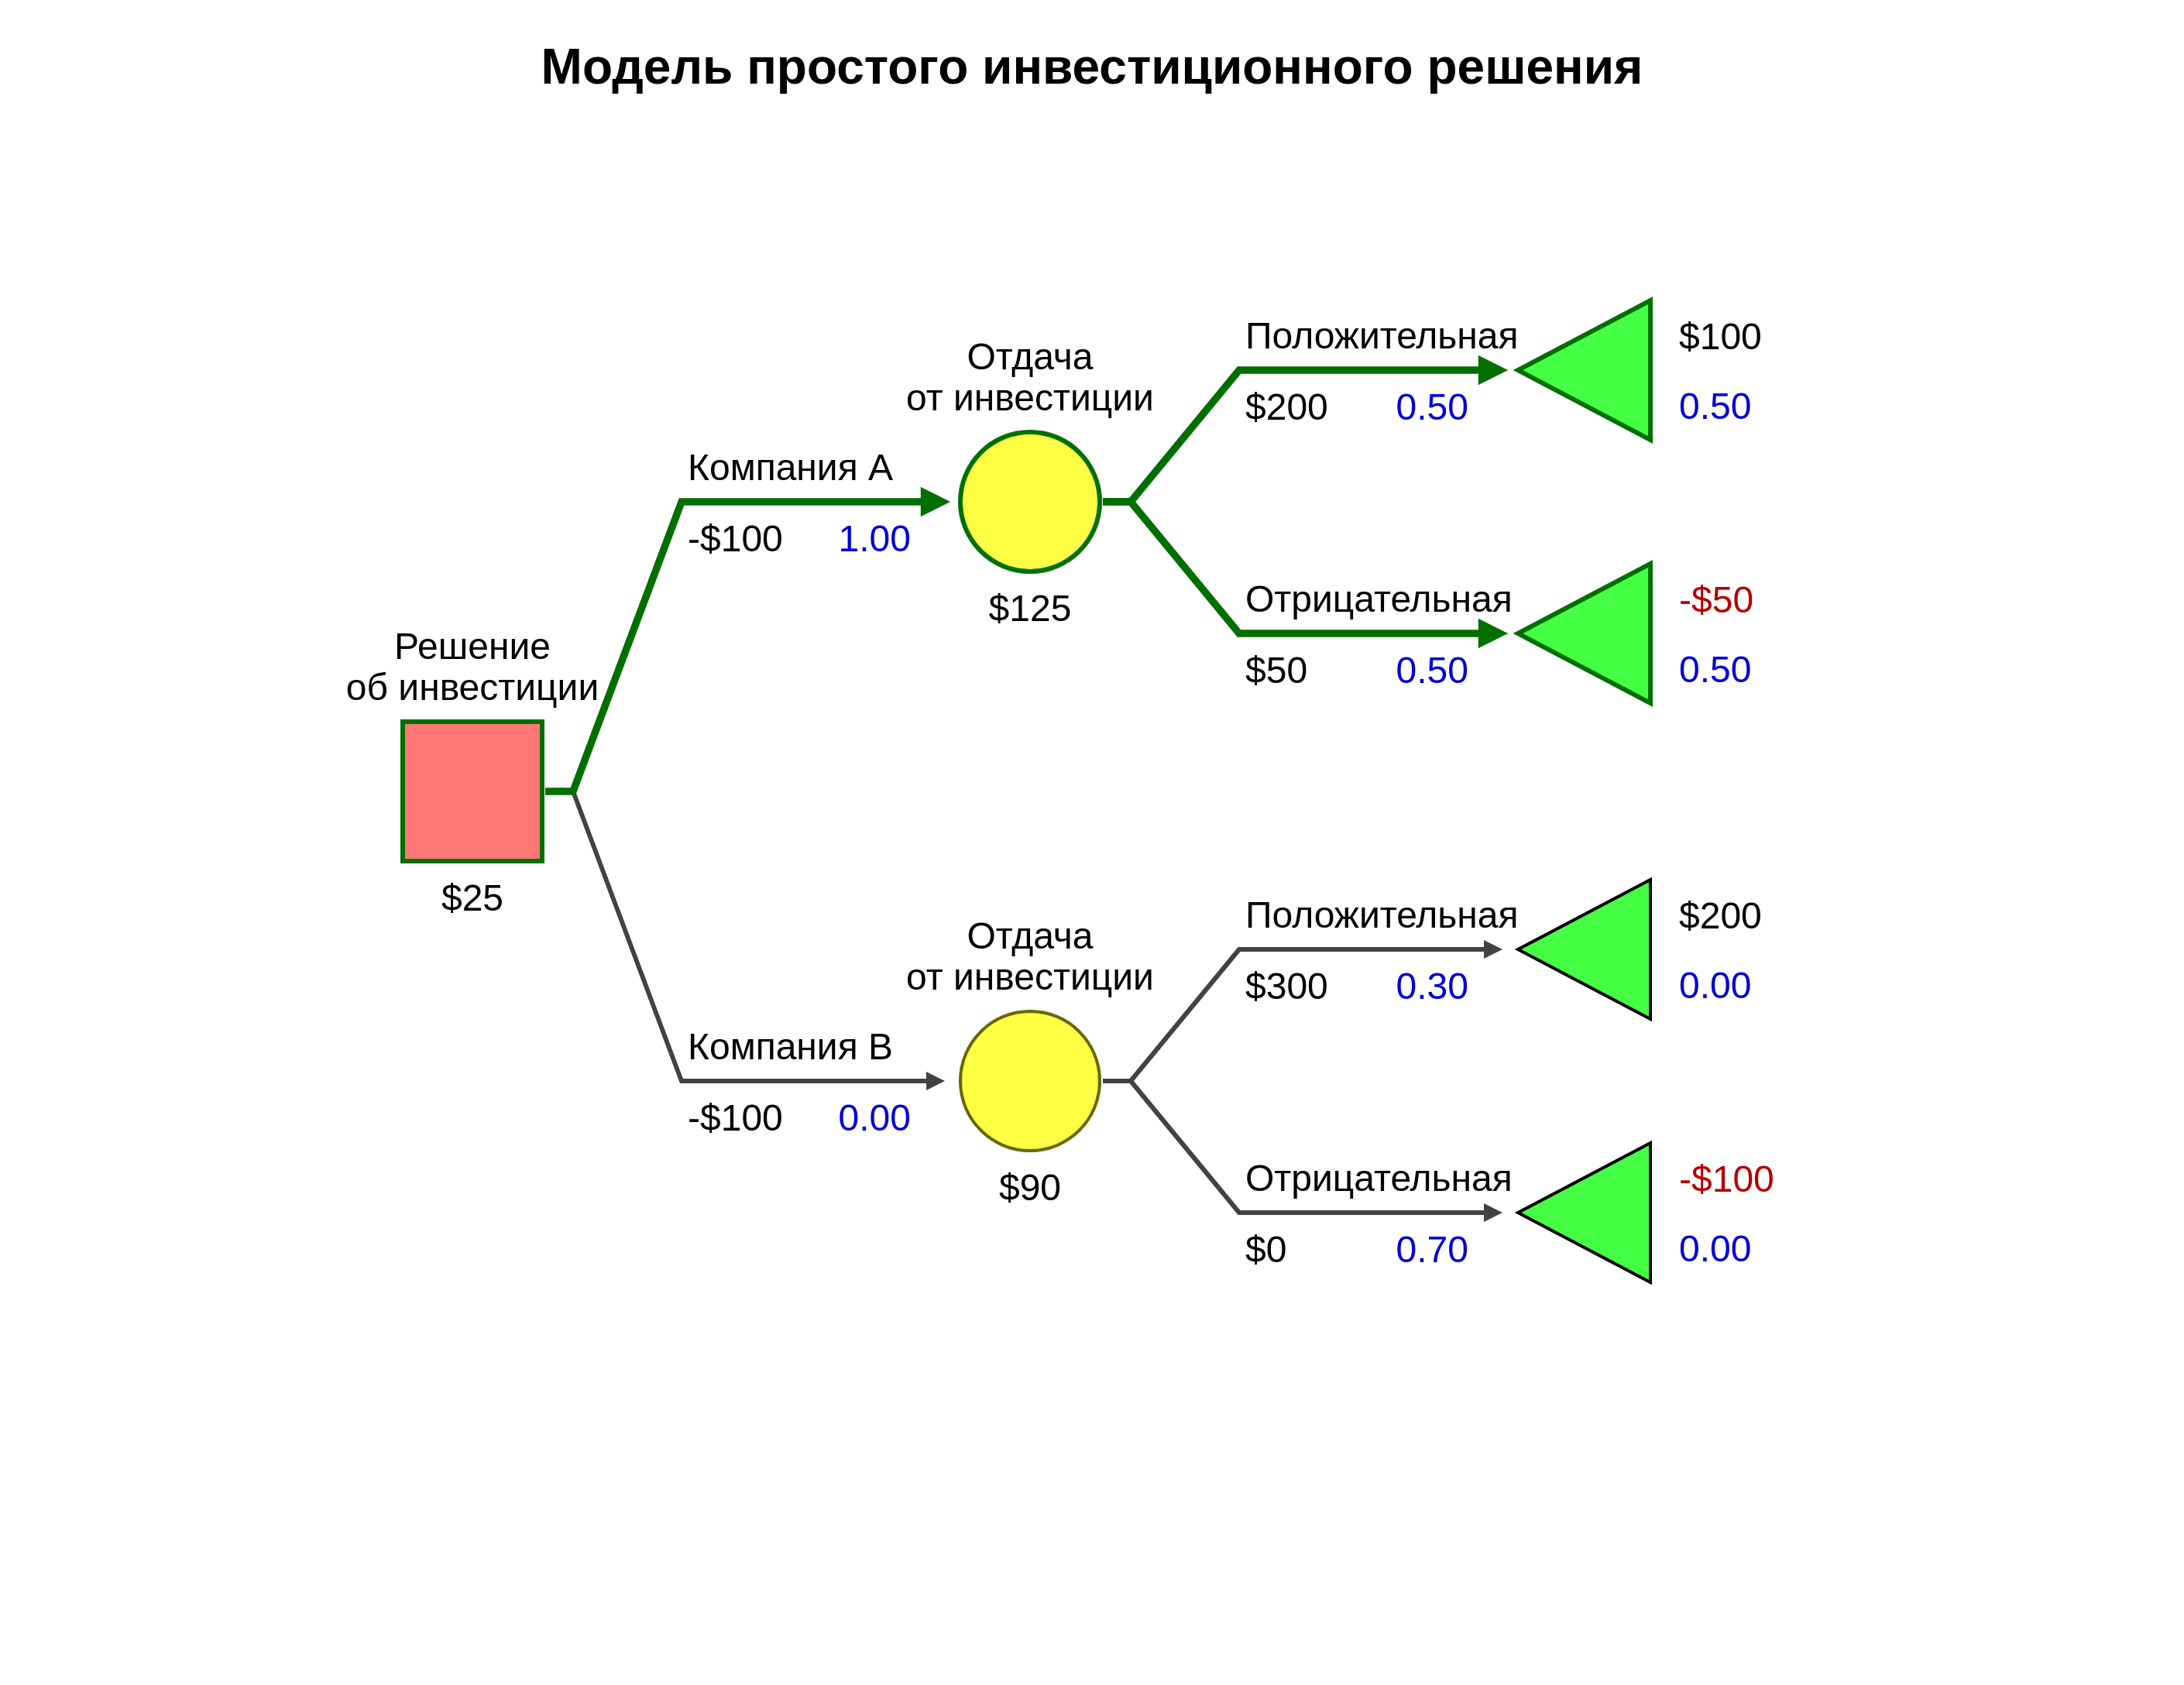
\includegraphics[width= 15cm]{pics/simple_decision_tree_1.png} 
	\label{fig:sample}
	\caption{Простое дерево решений}
\end{figure}

Модель дерева решений описывает и визуализирует последовательность принятия решения в условиях неопределенности на древовидной диаграмме. Это означает, что деревья решений могут быть полезны в таких задачах:
\begin{itemize}
    \item лицо, принимающее решение, выполняет несколько действий, следуя друг за другом,
    \item состояния мира могут различаться в зависимости от уже принятых решений,
    \item некоторые решения могут привести к более точным оценкам вероятности этих состояний.
\end{itemize}

На древовидной диаграмме представлены возможные решения, которые необходимо принять, независимые события, которые могут произойти, и результаты, связанные с комбинациями этих решений и событий. Необходимо определить два параметра: вероятности событий и их значения или стоимости. Первый параметр представляет вероятность получения определенного состояния мира. Поскольку возможные состояния мира в рамках одной реакции на самом деле являются конкурирующими событиями, сумма их вероятностей должна быть равна 1. 
Тогда значения или стоимости, выраженные в некоторой шкале, например в деньгах, означают платежи (изменение стоимости) как следствие решения или состояния мира. 
Это может быть как прибыль, так и убытки. Модель дерева решений включает еще одно понятие: EMV - ожидаемая значение или ожидаемая ценность (или ожидаемая полезность). Она вычисляется как вероятностно-взвешенное среднее значений для конкурирующих наборов решений и событий. Ожидаемое значение EMV показывает, сколько человек может заработать или потерять, принимая оптимальные решения (это означает такие решения, которые максимизируют прибыль и минимизируют убытки). Наконец, результат, связанный с решениями и событиями, представляет собой общее последствие набора решений и событий во всем процессе принятия решения. Он может быть истолкован как отдача лица, принимающего решение - результат как его решений, так и произошедших независимых событий.

Деревья решений с их простой для понимания структурой являются отличным инструментом для решения задач анализа. Они позволяют исследовать возможные результаты принятия решений и помогают выбирать между различными направлениями действий. Основной целью модели дерева решений является определение наилучшей возможной политики, которая представляет собой наибольшую отдачу или наименьший убыток.


Дерево решений строится по направленному графику слева направо, с набором узлов, которые разбиваются на три разрозненных множества:
\begin{itemize}
    \item узлы решения - типично представленные в виде квадратов,
    \item случайные узлы, представленные в виде кругов,
    \item терминальные узлы представлены в виде треугольников.
\end{itemize}

Крайняя левая вершина называется корневой вершиной и является первой вершиной принятия решения (первый красный квадрат слева - см. выше простую модель принятия инвестиционного решения - рисунок \ref{fig:sample} ). В узлах принятия решений выбирает именно тот, кто принимает решение, т.е. выбирает ровно одну из ветвей, выходящих из этого узла. Эти ветви представляют собой набор доступных альтернатив решения (действий). В случайном узле (желтые кружки - дерево образцов выше) каждая из вытекающих из него ребер - реакция - выбирается случайным образом с заданной вероятностью события. Терминальные узлы (синие треугольники на дереве выборки выше) представляют собой результат последовательности действий/реакций от корневого узла к данному конкретному терминальному узлу. Терминальный узел является конечной точкой: никакие решения не могут быть приняты, и никакие события не могут произойти после этого.

В приложении SilverDecisions вероятность событий и значения, связанные с этими событиями или решениями, определяются по краям. Ожидаемые значения, рассчитанные для каждого набора решений/событий, отображаются в каждом узле решения/шанса, а терминальные узлы показывают результаты и вероятности того, что событие окажется в указанном терминальном узле.

Обратите внимание, что каждое ребро совмещается с двумя узлами: левый, из которого выходит ребро, называется родительским узлом, а второй, находящийся справа, называется дочерним узлом. Поддерево - это еще один термин, связанный с деревьями решений - оно представляет собой ту часть дерева, которая начинается в любом дочернем узле, и каждый из них вместе с любыми потомками образует поддерево. Например, поддерево, уставившееся в корневой узел, представляет собой целое дерево.






\section{Задачи с примерами решения}

Деревья решений являются удобным инструментом для формализации процесса принятия решений. Они достаточно широко используются в нефтяной индустрии [привести ссылки на книгу и статьи]. 

Для построения деревьев решений можно использовать ручку, бумагу и калькулятор, так расчеты достаточно просты. Но удобнее использовать специализированные программные инструменты. Далее мы будем использовать сайт \url{http://silverdecisions.pl/} предоставляющий удобный, и что не менее важно, бесплатный и открытый программный комплекс для построения и анализа деревьев решений.

\subsection{Исследования на разведочной скважине}
    
    
Оцените стоит ли проводить комплекс исследований на разведочной скважине со следующими параметрами:
\begin{itemize}
    \item Стоимость 1 млн руб
    \item Ожидаемая информация – фильтрационные параметры пласта, уточнение строение пласта
    \item Вероятность успешности исследования (получения какой то информации) 70%
    \item Ожидается что исследование подтвердит увеличение запасов на 15% (60% что запасы увеличатся)
    \item Текущие извлекаемые запасы – 1 млн т. нефти, стоимость 1 т.нефти в запасах – 1 тыс. руб.
\end{itemize}     
Стоит ли проводить исследование? 

    
\subsection{КВД на добывающей скважине}

Оцените стоит ли проводить КВД на эксплуатационной скважине с дебитом 50 т/нефти, Рзаб = 50 атм, Рпл = 250 атм
\begin{itemize}
    \item Стоимость исследования 1 млн руб
    \item Длительность 1 неделя (скважина остановлена)
    \item Ожидаемая информация – фильтрационные параметры пласта, скин фактор
    \item Вероятность успешности исследования (получения какой то информации) 70%
    \item Ожидается что исследование подтвердит наличие положительного скин фактора
    \begin{itemize}
        \item S=0 с вероятностью 50%
        \item S=5 с вероятностью 40%
        \item S=15 с вероятностью 10%
    \end{itemize}
    \item Стоимость кислотной обработки снижающей скин в 2 раза 1 млн руб. Длительность эффекта 1 год
    \item Стоимость нефти 1 т = 10 тыс. руб.
\end{itemize}
Стоит ли проводить исследование? 

\subsection{Исследование фонтанирующей скважины}
Имеется фонтанирующая скважина. Дебит нефти 30 т/сут. Воды нет. Имеется водоносный пласт под продуктивным. Перемычка 10 м. Вероятность получения прорыва воды после ГРП 50 \%. При прорыве воды рост обводненности до 90 \% без увеличения дебита нефти. Без прорыва воды увеличение продуктивности в 3 раза. Стоимость ГРП 1 млн. руб.

Оценить что делать на скважине?

Ничего не делать
Сделать ГРП
Провести исследование и по его результатам ГРП
Стоимость исследования 100 т.р.

Вероятность выявления скважины где ГРП будет успешен 60%

\chapter{Промысловые исследования}

Здесь основные определения и теоретический минимум для последующих разделов. 
И набор мелких "коварных" задач для контроля знаний.
\section{Теория и определения}
\begin{itemize}
    \item Пластовые флюиды. Вода, нефть, газ.
    \item Модели флюидов. Модель нелетучей нефти. Композиционная модель. Основные предположения и отличия
    \item Параметры нефти для модели нелетучей нефти. Из зависимость от давления и температуры. 
    \item Параметры газа. z фактор. Коэффициент Джоуля Томсона для углеводородных газов. 
    \item Параметры воды и пара.
    
\end{itemize}
\section{Методы определения свойств флюидов}
Отбор глубинных проб, замеры на поверхности. Экспресс методы исследования.
\section{Задачи}
Расчеты с использованием Excel, Python, специализированное ПО
\begin{itemize}
    \item Зависимости параметров нефти воды и растворенного газа от давления и температуры (можно с использованием унифлок Excel)
    \item Построить график плотности воды при одновременно изменяющихся давлении и температуре
    \item Построить график зависимости доли свободного газа  от давления и температуры в потоке
    \item Оценить изменение температуры газа и ГЖС при изменении давления из за эффекта Джоуля Томсона
    \item Рассчитать изменение свойств воды и пара при нагреве.
    \item оценка газового фактора по данным замера расхода газа и нефти - учет растворенного в нефти газа на замерной с высоким давлением.

    % недавно было обнаружено что график достаточно странно выглядит :) 
    %\item Расчеты закона Дарси для трубы и простые задачи по линейному потоку в пласте. Определить перепад давления в трубе, оценить скорость движения жидкости и так далее.
\end{itemize}
    

\section{Барометрические исследования и расчет распределения давления в скважине и трубопроводах}

Давление - ключевой параметр в системе пласт - скважина - скважинное оборудование. Перепад давления вызывает движение флюидов. Давлением можно управлять с помощью оборудования. Поэтому замеры давления и исследования построенные на контроле давления - ключевые для нефтедобычи.

Поскольку нефть и пластовые флюиды транспортируются по трубам - то изучение многофазного потока в трубах и скважинах занимает заметное место в управлении добычей. На моделировании этих процессов основан ряд методов исследования. 

В этом разделе посмотрим некоторые подходы к моделированию систем нефтедобычи и проведению исследований этих систем связанных с замерами давления.

\subsection{Теория}
\begin{itemize}
    \item Измерение давлений - датчики и принципы. Краткий обзор и ссылки. Принципы измерения давления, температурная компенсация, Приборы для измерения давления в эксплуатируемой скважине
    \item Связь давления и движения флюидов в трубах и скважине. Формула Дарси-Вейсбаха, уравнение Навье Стокса. Важность учета PVT при моделировании потоков
    \item Методы расчета распределения давления в потоке. Краткой обзор методов и программ. Примеры расчета.
    \item 
\end{itemize}

\subsection{Методы исследования с использованием измерений давления}
\begin{itemize}
    \item Забойное давление - ключевой параметр для контроля работы скважины. Методы контроля забойного давления - прямые измерения и косвенные оценки для различных типов скважин. Частота измерения забойного давления. Цели и задачи измерения забойного давления.
    \item Хранение результатов измерений давления. Шахматка, Техрежим, БСИ ЭЦН, корпоративные базы данных.
    \item Барометрия в работающей скважине
    \item Оценка параметров работы заглушенных скважин
\end{itemize}

\subsection{Задачи}

Задачи с использованием Excel и пакетов программ. 

\begin{itemize}
    \item Расчет распределения давления в скважине с использованием гидравлических корреляций. Построение кривой распределения давления в скважине.
    \item Расчет забойного давления по динамическому уровню в скважине с ЭЦН. Анализ отжима динамического уровня. 
    \item Оценка пластового давления в заглушенной скважине
\end{itemize}


\section{Термометрические исследования и расчет распределения температуры потока в скважине и трубопроводах}

\subsection{Теория}
\begin{itemize}
    \item Теория по замеру температуры в стволе скважины и в потоке
    \item Принципы измерения температуры и датчики температуры
\end{itemize}


\subsection{Методы исследования с использованием измерений температуры}

\begin{itemize}
    \item Термометрия в стволе скважины. Расчет температуры на устье. Выявление зон опасных для отложения парафинов гидратов
    
    \item Термометрия в продуктивном интервале 
    
    \item Термометрия в газлифтной скважине для анализа работы газлифтных клапанов
    
    \item Температурный режим работы ЭЦН. Предотвращение отказов ЭЦН на основе замеров температуры
\end{itemize}

\subsection{Задачи}

Задачи с использованием Excel и пакетов программ. 

\begin{itemize}
    \item Расчет распределения температуры в скважине с учетом притока разных флюидов в скважине
    \item Калориметрическое смешивание
    \item Расчет распределения температуры в газлифтной скважине
    \item Расчет температурного режима работы ЭЦН
    \item Расчет температуры и отложение гидратов
    
\end{itemize}


% хороший раздел - но тут сложно придумать хорошие задачи 
% на практике дебитам либо верим и используем, либо не верим
% дебитограммы никто нынче особо не смотрит 
% хотя можно сделать блок по построению дебитограмм из синтетических данных
% и примеры с интерпретацией соответственно 
\section{Теория}
\begin{itemize}
    \item Принципы измерения дебита (расхода). Оборудования для измерения дебита на поверхности и в скважине
    \item Замер обводненности и газового фактора продукции
    \item Замеры количества механических примесей
    \item Профили притока к скважине. Замер профиля притока с использованием скважинного оборудования
\end{itemize}

\section{Задачи}

\begin{itemize}
    \item Оценка дебита по закону Бернулли - на гидравлическом сужении. Оценка дебита по характеристике потока через штуцер
    \item Оценка обводненности по данным замером плотности флюидов и плотности смеси
    \item Оценка газового фактора по данным эксплуатации скважины - перепад давления в скважине и на штуцере
    \item Оценка газового фактора по данным отжима динамического уровня
    \item Расчет профиля изменения давления и профиля притока в горизонтальной скважине (учет по плотности притока и диаметру ствола скважины)
    
\end{itemize}
%\section{Выявление нарушений герметичности ствола скважины}
    

\chapter{Гидродинамические исследования}


\section{Гидродинамические исследования скважин и пластов}


В основе гидродинамических исследований скважин и пластов, как и для других видов исследований, лежит сопоставление результатов измерений на скважинах с математическими моделями их работы. Используются различные виды измерений - дебиты по фазам, давления на устье и забое, динамика изменения параметров во времени. Если найти такую модель, которая объясняла бы наблюдаемые изменения параметров, тогда можно надеяться, что она сможет дать хороший прогноз.

Необходимость сопоставления измерений с моделями требует детального понимания того как устроены модели. Месторождение, продуктивный пласт, скважины - являются сложными объектами работу которых определяет множество факторов и физических процессов. Построение единой детальной модели, способной учесть всю доступную информацию - на практике оказывается чрезвычайно сложной задачей. Попытка построить такую модель неизбежно приводит к тому, что для учета всей имеющейся информации в модель приходится вносить большой объем данных и еще больше догадок и предположений (не упоминая даже того, что и в имеющейся информации мы часто не очень то уверены). Это приводит к тому, что прогноз (и решения зависящие от него) могут оказаться неверными. 

Вместо одной супер модели на практике более эффективно применять иерархию моделей. Для каждой задачи, можно подобрать отдельную, относительно простую модель позволяющую принять необходимое решение. Хорошо иллюстрирует подход к выбору модели афоризм -- модель должна быть максимально простой - но не проще чем необходимо. 

Применяя иерархию моделей, важным становится понимать как устроены разные модели, начиная от самых простых - и далее с различными усложнениями, и дополнительными эффектами.

Этот раздел посвящен разбору простых моделей фильтрации, которые лежат в основе методов интерпретации гидродинамических исследований.

\section{Теоретические основы}

\subsection{Уравнение фильтрации}

Уравнение фильтрации многофазного потока в пористой среде - основная математическая модель пласта используемая в инженерных приложениях. Используется не само уравнение, а разнообразные частные решения, описывающие те или иные ситуации. Наиболее широко известным примером решения уравнения фильтрации, возможно является, численное решение которое строится трехмерными гидродинамическими симуляторами (eclipse, tnavigator и так далее)

%[[Вывод уравнения фильтрации]]

Как правило, при выводе уравнения фильтрации используются следующие соотношения:

закон Дарси:  

\begin{equation} \label{eq:darcy_law_1}
 u_r=-\frac{k}{\mu}\frac{dp}{dr} 
\end{equation}

уравнение неразрывности: 
\begin{equation} \label{eq:mass_balance_1} 
\frac{1}{r}\frac{\partial\left(r\rho u_r\right)}{\partial r}=-\varphi\frac{\partial p}{\partial t} 
\end{equation}

уравнение состояния: 
\begin{equation} \label{eq:eos_1} 
c_0=\frac{1}{\rho}\frac{\partial\rho}{\partial p} 
\end{equation}

Опираясь на эти соотношения уравнение фильтрации в радиальной форме можно привести к виду.

\begin{equation} \label{eq:diff_eq_1} 
\frac{\partial ^2 p }{\partial r^2} + \frac{1}{r} \frac{\partial p}{\partial r} = \frac{\varphi \mu c_t}{k} \frac{\partial p}{\partial t} 
\end{equation}

Здесь используются следующие обозначения

$u_r$ - скорость фильтрации в направлении $r$, м/сек

$k$ - проницаемость, м$^2$

$\mu$ - вязкость флюида, Па с

$p$ - давление, Па 

$r$ - расстояние, м 

$\rho$ - плотность флюида, кг/м$^3$

$\varphi$ - пористость породы, доли единиц.

$c_t$ - общая сжимаемость породы и флюида, 1/Па

\subsection{Вывод уравнения фильтрации}


Вывод уравнения фильтрации основан на следующих предположениях: 
\begin{itemize}
	\item пласт однородный и изотропный - пористость и проницаемость одинаковы во всем пласте и во всех направлениях и не зависят от давления 
	\item добывающая скважина вскрывает весь продуктивный горизонт и обеспечивает радиальный приток к скважине
	\item пласт насыщен одним флюидом на всем протяжении
	\item температура не меняется в пласте, изотермичность
\end{itemize}

Схема притока приведена на рисунке \ref{ris:radial_inflow_scheme}.

\begin{figure}[h!]
	\begin{center}
		

\tikzset{every picture/.style={line width=0.75pt}} %set default line width to 0.75pt        

\begin{tikzpicture}[x=0.75pt,y=0.75pt,yscale=-1,xscale=1]
%uncomment if require: \path (0,300); %set diagram left start at 0, and has height of 300

%Shape: Ellipse [id:dp024533754320974488] 
\draw  [fill={rgb, 255:red, 243; green, 237; blue, 161 }  ,fill opacity=1 ] (255.9,210) .. controls (255.9,198.95) and (298.25,190) .. (350.5,190) .. controls (402.75,190) and (445.1,198.95) .. (445.1,210) .. controls (445.1,221.05) and (402.75,230) .. (350.5,230) .. controls (298.25,230) and (255.9,221.05) .. (255.9,210) -- cycle ;
%Shape: Can [id:dp18120956683853207] 
\draw  [fill={rgb, 255:red, 243; green, 237; blue, 161 }  ,fill opacity=1 ] (365.5,176.25) -- (365.5,210) .. controls (365.5,212.49) and (358.78,214.5) .. (350.5,214.5) .. controls (342.22,214.5) and (335.5,212.49) .. (335.5,210) -- (335.5,176.25) .. controls (335.5,173.76) and (342.22,171.75) .. (350.5,171.75) .. controls (358.78,171.75) and (365.5,173.76) .. (365.5,176.25) .. controls (365.5,178.74) and (358.78,180.75) .. (350.5,180.75) .. controls (342.22,180.75) and (335.5,178.74) .. (335.5,176.25) ;
%Shape: Ellipse [id:dp0014041786513778742] 
\draw  [fill={rgb, 255:red, 243; green, 237; blue, 161 }  ,fill opacity=1 ] (255.9,167.25) .. controls (255.9,156.2) and (298.25,147.25) .. (350.5,147.25) .. controls (402.75,147.25) and (445.1,156.2) .. (445.1,167.25) .. controls (445.1,178.3) and (402.75,187.25) .. (350.5,187.25) .. controls (298.25,187.25) and (255.9,178.3) .. (255.9,167.25) -- cycle ;
%Shape: Can [id:dp09417665438601963] 
\draw  [fill={rgb, 255:red, 243; green, 237; blue, 161 }  ,fill opacity=1 ] (365.5,62) -- (365.5,167.25) .. controls (365.5,169.74) and (358.78,171.75) .. (350.5,171.75) .. controls (342.22,171.75) and (335.5,169.74) .. (335.5,167.25) -- (335.5,62) .. controls (335.5,59.51) and (342.22,57.5) .. (350.5,57.5) .. controls (358.78,57.5) and (365.5,59.51) .. (365.5,62) .. controls (365.5,64.49) and (358.78,66.5) .. (350.5,66.5) .. controls (342.22,66.5) and (335.5,64.49) .. (335.5,62) ;
%Straight Lines [id:da05427875829374096] 
\draw    (255.9,167) -- (255.9,210) ;
%Straight Lines [id:da08444018377929519] 
\draw    (445.1,167) -- (445.1,210) ;
%Straight Lines [id:da7446827946920336] 
\draw    (475,170) -- (475,207) ;
\draw [shift={(475,210)}, rotate = 270] [fill={rgb, 255:red, 0; green, 0; blue, 0 }  ][line width=0.08]  [draw opacity=0] (8.93,-4.29) -- (0,0) -- (8.93,4.29) -- cycle    ;
\draw [shift={(475,167)}, rotate = 90] [fill={rgb, 255:red, 0; green, 0; blue, 0 }  ][line width=0.08]  [draw opacity=0] (8.93,-4.29) -- (0,0) -- (8.93,4.29) -- cycle    ;
%Straight Lines [id:da9533475438509436] 
\draw    (309.1,152.25) -- (325.75,159) ;
\draw [shift={(327.6,159.75)}, rotate = 202.07] [color={rgb, 255:red, 0; green, 0; blue, 0 }  ][line width=0.75]    (6.56,-2.94) .. controls (4.17,-1.38) and (1.99,-0.4) .. (0,0) .. controls (1.99,0.4) and (4.17,1.38) .. (6.56,2.94)   ;
%Straight Lines [id:da7628148018069294] 
\draw    (310.6,179.75) -- (327.72,173.44) ;
\draw [shift={(329.6,172.75)}, rotate = 519.78] [color={rgb, 255:red, 0; green, 0; blue, 0 }  ][line width=0.75]    (6.56,-2.94) .. controls (4.17,-1.38) and (1.99,-0.4) .. (0,0) .. controls (1.99,0.4) and (4.17,1.38) .. (6.56,2.94)   ;
%Straight Lines [id:da8513852103635728] 
\draw    (387.6,181.75) -- (370.31,173.6) ;
\draw [shift={(368.5,172.75)}, rotate = 385.23] [color={rgb, 255:red, 0; green, 0; blue, 0 }  ][line width=0.75]    (6.56,-2.94) .. controls (4.17,-1.38) and (1.99,-0.4) .. (0,0) .. controls (1.99,0.4) and (4.17,1.38) .. (6.56,2.94)   ;
%Straight Lines [id:da03702921414833504] 
\draw    (391.1,154.75) -- (375.89,160.09) ;
\draw [shift={(374,160.75)}, rotate = 340.66999999999996] [color={rgb, 255:red, 0; green, 0; blue, 0 }  ][line width=0.75]    (6.56,-2.94) .. controls (4.17,-1.38) and (1.99,-0.4) .. (0,0) .. controls (1.99,0.4) and (4.17,1.38) .. (6.56,2.94)   ;
%Straight Lines [id:da15593017089479355] 
\draw    (350.5,50.67) -- (350.5,32) ;
\draw [shift={(350.5,30)}, rotate = 450] [color={rgb, 255:red, 0; green, 0; blue, 0 }  ][line width=0.75]    (6.56,-2.94) .. controls (4.17,-1.38) and (1.99,-0.4) .. (0,0) .. controls (1.99,0.4) and (4.17,1.38) .. (6.56,2.94)   ;

% Text Node
\draw (258.9,182.73) node [anchor=north west][inner sep=0.75pt]    {$k$};
% Text Node
\draw (370.67,126.98) node [anchor=north west][inner sep=0.75pt]    {$P_{wf}$};
% Text Node
\draw (478,181.73) node [anchor=north west][inner sep=0.75pt]    {$h$};
% Text Node
\draw (369.33,61.07) node [anchor=north west][inner sep=0.75pt]    {$r_{w}$};


\end{tikzpicture}
		\caption{Схема радиального притока к скважине}
		\label{ris:radial_inflow_scheme}
	\end{center}
\end{figure}

Используются следующие обозначения параметров:

\(h\) - толщина пласта

\(k\) - средняя проницаемость

\(r\) - радиус (расстояние от скважины)

\(r_e\) -  внешний радиус зоны дренирования

\(r_w\) - радиус скважины

\(p\) - давление

\(q\) - объемный расход флюида в рабочих условиях - дебит

\(t\) - время

\(u_r\) - приведенная скорость

\(\varphi\) -  пористость

\(\mu\) - вязкость

\(\rho\) - плотность флюида

\subsubsection{Радиальная модель притока}
Уравнение фильтрации или уравнение движения флюидов основывается на принципах сохранения массы и импульса (количества движения). Для жидкости закон сохранения импульса принимает форму закона Дарси. При этом эффекты турбулентности и отклонения потока от Дарси не учитываются. Они важны для газовых скважин и могут быть введены в уравнение фильтрации отдельно. 

Закон сохранения массы или принцип неразрывности можно выразить в радиальной форме следующим соотношением

\begin{equation} \label{eq:mass_balance_2}
\frac{1}{r}\frac{\partial\left(r\rho u_r\right)}{\partial r}=-\varphi\frac{\partial p}{\partial t}
\end{equation}

Принцип неразрывности показывает, что для определенного объема пласта, масса флюида которое втекла в контрольный объем пласта минус масса которая вытекла равна массе которая накопилась в объеме. 

Сохранение импульса или закон Дарси можно выразить соотношением  


\begin{equation} \label{eq:darcy_law_2}
 u_r=-\frac{k}{\mu}\frac{d^p}{dr}
\end{equation}

Закон Дарси здесь используется как псевдоустановившаяся аппроксимация обобщенного уравнения сохранения импульса (то есть слагаемым отвечающим за накопление импульса пренебрегаем). Это предположение справедливо если не учитывать возмущения давления в среде двигающиеся со скоростью звука. Все изменения давления описываемые моделью связаны с локальными изменениями градиента давления за счет ламинарного режима потока. Хотя далее в модели будет учтена сжимаемость системы всеми "звуковыми" \ эффектами в системе мы пренебрегаем.

Поток предполагается горизонтальным, поэтому давление \( p\) может быть использовано в качестве потенциала потока, гравитационными силами пренебрегаем.

Комбинируя уравнения (\ref{eq:mass_balance_2}), (\ref{eq:darcy_law_2})  получим:

\begin{equation} \label{eq:diff_eq_2}
\frac{1}{r}\frac{\partial\left( \dfrac{r\rho k}{\mu}\dfrac{\partial p}{dr}\right)}{\partial r}=\varphi\frac{\partial \rho}{\partial t}
\end{equation}

Уравнение (\ref{eq:diff_eq_2}) -- дифференциальное уравнение в частных производных описывающее нестационарный поток однофазного флюида в пористой среде при ламинарном потоке. 

Вообще говоря приведенное уравнение является нелинейным, так как плотность $\rho = \rho(p)$ и вязкость $\mu = \mu(p)$ являются функциями давления. Уравнение содержит две зависимые переменные - давление $p$ и плотность $\rho$. Поэтому для его решения необходимо задать еще одно соотношение, каковым может быть уравнение состояния флюида связывающее плотность флюида и давление $\rho = \rho(p)$. 

\subsubsection{Флюид постоянной сжимаемости}
 
Нестационарное поведение давления в пласте связано со сжимаемостью системы. При изменении давления в какой то точке, часть флюида сжимается, происходит накопление или отдача флюида, что вызывает задержку в распространении изменения флюида. Несмотря на то, что сжимаемость флюидов и породы малы и во многих случаях ими можно пренебречь, это не верно для пластовых систем для добычи нефти. Большие объемы пласта и флюидов и высокие давления компенсируют малость сжимаемости и требуют ее учета. 

Для однофазного флюида разумным является предположение постоянства сжимаемости.

Сжимаемость можно определить как 

$$c=-\frac{1}{V} \left(  \frac{ \partial V}{ \partial p}  \right) $$ 

учтем, что

$$ \rho = \frac{m}{V} $$  

тогда получим

$$c=\frac{1}{\rho} \left(  \frac{ \partial \rho}{ \partial p}  \right) $$ 

Для флюида с постоянной сжимаемостью, проинтегрировав приведенное уравнение можно получить 

$$\rho = \rho_i e^{c(p-p_i)}$$

где $\rho_i$ плотность флюида при некотором заданном давлении $p_i$

Продифференцировав выражение для плотность по времени получим 

$$
c \rho \frac{\partial p}{\partial t} = \frac{\partial \rho}{\partial t}
$$

Подставив это выражение в ранее полученное уравнение фильтрации получим 

$$ 
\frac{1}{r}\frac{\partial\left( \dfrac{r\rho k}{\mu}\dfrac{\partial p}{dr}\right)}{\partial r}=\varphi c \rho \frac{\partial p}{\partial t}  
$$

Приведенное дифференциальное уравнение в частных производных все еще нелинейно, поскольку зависит от плотности $\rho$ 



\subsubsection{Общая сжимаемость}
Если пористость не является постоянной величиной и меняется с давлением, тогда  слагаемое отвечающее за накопление флюида в пласте можно выразить как 


$$\frac{\partial \varphi \rho}{\partial t} = \varphi \frac{\partial \rho}{\partial t}+ \rho \frac{\partial \varphi }{\partial t} = \varphi c_l \rho \frac{\partial p}{\partial t} + \rho \frac{\partial \varphi }{\partial t}  $$

где $c_l$ сжимаемость жидкости. 

Определим сжимаемость породы как 

$$c_f = \frac{1}{\varphi} \frac{\partial \varphi}{\partial p}$$

тогда 

$$\frac{\partial \varphi \rho}{\partial t}  = \varphi \rho (c_l + c_f) \frac{\partial p}{\partial t}   $$



хотя пористость здесь является функцией давления - в первом приближении мы можем считать ее константой равной пористости при некотором среднем давлении в пласте. Это справедливо для маленькой сжимаемости породы, что верно почти всегда.

Уравнение для сжимаемости можно еще уточнить, учтя что в пласте могут находится различные флюиды - вода и нефть с насыщенностями  $s_w$ и $s_o$

тогда 

$$ c_l = s_o c_o + s_w c_w $$

тогда можно ввести общую сжимаемость системы 

$$ c_t = c_l + c_f = s_o c_o + s_w c_w  + c_f $$ 

Заметим, что проницаемость k в законе Дарси это не абсолютная проницаемость, но относительная проницаемость по нефти при насыщенности водой соответствующей связанной воде.  

$$ k= k_o (s_{wc}) $$

\subsubsection{Линеаризация уравнения фильтрации}

Раскрыв производную в левой части уравнения и предположив, что $\dfrac{\partial p}{\partial r}$ мало а следовательно слагаемым  $ r \rho c_t \left( \dfrac{\partial p}{\partial r} \right)^2 $ можно пренебречь, что приведет к линеаризации уравнения фильтрации

$$ \frac{\partial^2 p}{\partial r^2} + \frac{1}{r} \frac{\partial p}{\partial r}= \frac{\varphi \mu c_t}{k} \frac{\partial p}{\partial t} $$



\subsection{Стационарные решения уравнения фильтрации}

Широкое распространение на практике получили стационарные решения уравнения фильтрации. Приведем некоторые из них.

\subsubsection{Решение для постоянного давления на границе}

Рассматривается самая простая модель работы добывающей скважины - радиальная стационарная фильтрация в однородном изотропном пласте. 
Уравнение фильтрации описывается законом Дарси, который должен быть приведен к радиальной форме и в таком варианте известен как Формула Дюпюи.  В простейшем случае рассматривается модель с поддержанием давления на круговом контуре питания скважины радиусом $r_e$ (рисунок \ref{ris:radial_inflow_steady_state_1}).

\begin{figure}[h!]
	\begin{center}
		

\tikzset{every picture/.style={line width=0.75pt}} %set default line width to 0.75pt        

\begin{tikzpicture}[x=0.75pt,y=0.75pt,yscale=-1,xscale=1]
%uncomment if require: \path (0,493); %set diagram left start at 0, and has height of 493

%Shape: Rectangle [id:dp2210940442519349] 
\draw  [color={rgb, 255:red, 74; green, 144; blue, 226 }  ,draw opacity=1 ] (297.5,90) -- (432.5,90) -- (432.5,151) -- (297.5,151) -- cycle ;
%Shape: Circle [id:dp04970297189708517] 
\draw  [color={rgb, 255:red, 74; green, 144; blue, 226 }  ,draw opacity=1 ][fill={rgb, 255:red, 255; green, 255; blue, 255 }  ,fill opacity=1 ] (297.5,345) .. controls (297.5,307.72) and (327.72,277.5) .. (365,277.5) .. controls (402.28,277.5) and (432.5,307.72) .. (432.5,345) .. controls (432.5,382.28) and (402.28,412.5) .. (365,412.5) .. controls (327.72,412.5) and (297.5,382.28) .. (297.5,345) -- cycle ;
%Shape: Circle [id:dp10293196217835776] 
\draw   (247.5,345) .. controls (247.5,280.11) and (300.11,227.5) .. (365,227.5) .. controls (429.89,227.5) and (482.5,280.11) .. (482.5,345) .. controls (482.5,409.89) and (429.89,462.5) .. (365,462.5) .. controls (300.11,462.5) and (247.5,409.89) .. (247.5,345) -- cycle ;
%Shape: Rectangle [id:dp45852916067627625] 
\draw   (247.5,90) -- (482.5,90) -- (482.5,151) -- (247.5,151) -- cycle ;
%Shape: Rectangle [id:dp1911911198156271] 
\draw  [color={rgb, 255:red, 255; green, 255; blue, 255 }  ,draw opacity=1 ][fill={rgb, 255:red, 255; green, 255; blue, 255 }  ,fill opacity=1 ] (350,79.5) -- (380,79.5) -- (380,100.5) -- (350,100.5) -- cycle ;
%Shape: Circle [id:dp188351868386184] 
\draw   (350,345) .. controls (350,336.72) and (356.72,330) .. (365,330) .. controls (373.28,330) and (380,336.72) .. (380,345) .. controls (380,353.28) and (373.28,360) .. (365,360) .. controls (356.72,360) and (350,353.28) .. (350,345) -- cycle ;
%Straight Lines [id:da05843072951767869] 
\draw  [dash pattern={on 0.84pt off 2.51pt}]  (247.5,151) -- (247.5,345) ;
%Straight Lines [id:da5104578805624558] 
\draw  [dash pattern={on 0.84pt off 2.51pt}]  (482.5,151) -- (482.5,345) ;
%Straight Lines [id:da6468348992509316] 
\draw    (350,70) -- (350,90) ;
%Straight Lines [id:da34061741935451995] 
\draw    (380,70) -- (380,90) ;
%Straight Lines [id:da792017081317731] 
\draw  [dash pattern={on 0.84pt off 2.51pt}]  (365,90) -- (365,345) ;
%Straight Lines [id:da9746844382077546] 
\draw    (365,345) -- (430.75,436.32) ;
\draw [shift={(432.5,438.75)}, rotate = 234.25] [fill={rgb, 255:red, 0; green, 0; blue, 0 }  ][line width=0.08]  [draw opacity=0] (7.14,-3.43) -- (0,0) -- (7.14,3.43) -- cycle    ;
%Straight Lines [id:da25168233148692076] 
\draw    (365,345) -- (423.22,368.86) ;
\draw [shift={(426,370)}, rotate = 202.29] [fill={rgb, 255:red, 0; green, 0; blue, 0 }  ][line width=0.08]  [draw opacity=0] (7.14,-3.43) -- (0,0) -- (7.14,3.43) -- cycle    ;
%Straight Lines [id:da9459663069624791] 
\draw    (368,170) -- (429.5,170) ;
\draw [shift={(432.5,170)}, rotate = 180] [fill={rgb, 255:red, 0; green, 0; blue, 0 }  ][line width=0.08]  [draw opacity=0] (7.14,-3.43) -- (0,0) -- (7.14,3.43) -- cycle    ;
\draw [shift={(365,170)}, rotate = 0] [fill={rgb, 255:red, 0; green, 0; blue, 0 }  ][line width=0.08]  [draw opacity=0] (7.14,-3.43) -- (0,0) -- (7.14,3.43) -- cycle    ;
%Straight Lines [id:da9708245914645104] 
\draw    (368,192) -- (479.5,192) ;
\draw [shift={(482.5,192)}, rotate = 180] [fill={rgb, 255:red, 0; green, 0; blue, 0 }  ][line width=0.08]  [draw opacity=0] (7.14,-3.43) -- (0,0) -- (7.14,3.43) -- cycle    ;
\draw [shift={(365,192)}, rotate = 0] [fill={rgb, 255:red, 0; green, 0; blue, 0 }  ][line width=0.08]  [draw opacity=0] (7.14,-3.43) -- (0,0) -- (7.14,3.43) -- cycle    ;
%Straight Lines [id:da320252059166237] 
\draw    (365,70) -- (365,44.25) ;
\draw [shift={(365,41.25)}, rotate = 450] [fill={rgb, 255:red, 0; green, 0; blue, 0 }  ][line width=0.08]  [draw opacity=0] (7.14,-3.43) -- (0,0) -- (7.14,3.43) -- cycle    ;
%Straight Lines [id:da2674421622778862] 
\draw    (237,120.5) -- (255.2,120.5) ;
\draw [shift={(258.2,120.5)}, rotate = 180] [fill={rgb, 255:red, 0; green, 0; blue, 0 }  ][line width=0.08]  [draw opacity=0] (7.14,-3.43) -- (0,0) -- (7.14,3.43) -- cycle    ;
%Straight Lines [id:da8177707390860813] 
\draw    (286.9,120.5) -- (305.1,120.5) ;
\draw [shift={(308.1,120.5)}, rotate = 180] [fill={rgb, 255:red, 0; green, 0; blue, 0 }  ][line width=0.08]  [draw opacity=0] (7.14,-3.43) -- (0,0) -- (7.14,3.43) -- cycle    ;
%Straight Lines [id:da17218179619021767] 
\draw    (445.95,120.5) -- (422.1,120.5) ;
\draw [shift={(419.1,120.5)}, rotate = 360] [fill={rgb, 255:red, 0; green, 0; blue, 0 }  ][line width=0.08]  [draw opacity=0] (7.14,-3.43) -- (0,0) -- (7.14,3.43) -- cycle    ;
%Straight Lines [id:da6372180775348881] 
\draw    (495.93,120.5) -- (472.07,120.5) ;
\draw [shift={(469.07,120.5)}, rotate = 360] [fill={rgb, 255:red, 0; green, 0; blue, 0 }  ][line width=0.08]  [draw opacity=0] (7.14,-3.43) -- (0,0) -- (7.14,3.43) -- cycle    ;
%Straight Lines [id:da2394992655535546] 
\draw    (537,93) -- (537,148) ;
\draw [shift={(537,151)}, rotate = 270] [fill={rgb, 255:red, 0; green, 0; blue, 0 }  ][line width=0.08]  [draw opacity=0] (7.14,-3.43) -- (0,0) -- (7.14,3.43) -- cycle    ;
\draw [shift={(537,90)}, rotate = 90] [fill={rgb, 255:red, 0; green, 0; blue, 0 }  ][line width=0.08]  [draw opacity=0] (7.14,-3.43) -- (0,0) -- (7.14,3.43) -- cycle    ;

% Text Node
\draw (358.5,22.4) node [anchor=north west][inner sep=0.75pt]    {$q$};
% Text Node
\draw (383,68.4) node [anchor=north west][inner sep=0.75pt]    {$r_{w}$};
% Text Node
\draw (223.5,100.9) node [anchor=north west][inner sep=0.75pt]    {$q$};
% Text Node
\draw (276,100.9) node [anchor=north west][inner sep=0.75pt]    {$q$};
% Text Node
\draw (445.5,100.9) node [anchor=north west][inner sep=0.75pt]    {$q$};
% Text Node
\draw (495,100.9) node [anchor=north west][inner sep=0.75pt]    {$q$};
% Text Node
\draw (391,150.4) node [anchor=north west][inner sep=0.75pt]    {$r$};
% Text Node
\draw (450,170.4) node [anchor=north west][inner sep=0.75pt]    {$r_{e}$};
% Text Node
\draw (340.5,310.9) node [anchor=north west][inner sep=0.75pt]    {$r_{w}$};
% Text Node
\draw (413.5,349.4) node [anchor=north west][inner sep=0.75pt]    {$r$};
% Text Node
\draw (425,408.9) node [anchor=north west][inner sep=0.75pt]    {$r_{e}$};
% Text Node
\draw (485.5,165.9) node [anchor=north west][inner sep=0.75pt]    {$p_{e}$};
% Text Node
\draw (540,112.9) node [anchor=north west][inner sep=0.75pt]    {$h$};


\end{tikzpicture}
		\caption{Схема радиального притока к скважине при наличии постоянного давления на границе}
		\label{ris:radial_inflow_steady_state_1}
	\end{center}
\end{figure}


Для приведенной конфигурации можно записать закон Дарси в форме.

$$u_r=\frac{q}{2\pi rh}=\frac{k}{\mu}\frac{dP}{dr}$$

Проинтегрировав выражение по замкнутому контуру радиуса $r_e$ вокруг скважины можно выражение известное как формула Дюпюи
\marginpar{
	\href{https://qrgo.page.link/BqHRh}{Дюпюи, Жюль} 
	
\includegraphics[scale=0.4]{pics/qr_Dupuit.eps} 
}

\begin{equation} \label{eq:dupui_1}
q=\frac{2\pi kh\left(P_e-P_w\right)}{\mu\left(\ln{\dfrac{r_e}{r_w}}\right)}
\end{equation}


В приведенном выражения использованы единицы СИ. Здесь 

$u_r$ - приведенная скорость фильтрации на расстоянии $r$ от скважины, м/с 

$q$ - объемные дебит скважины в рабочих условиях, м$^3$/с

$r$ -  радиус - расстояние от центра скважины, м

$r_e$ -  радиус зоны дренирования, на котором поддерживается постоянное давление, м

$r_w$ - радиус скважины, на котором замеряется забойное давление, м

$P$ - давление, Па

$P_e$ - давление на внешнем контуре дренирования, Па

$P_w$ - давление на забое скважины, Па

$k$ - проницаемость, м$^2$

$\mu$ - вязкость нефти в зоне дренирования, Па с

На практике часто бывает удобнее пользоваться значениями в практических метрических единицах измерения. 

\begin{equation} \label{eq:dupui_2}
q=\frac{kh\left(P_e-P_w\right)}{ 18.41 \mu\left(\ln{\dfrac{r_e}{r_w}}\right)}
\end{equation}

где 

$q$ - объемные дебит скважины в рабочих условиях, м$^3$/сут

$r$ -  радиус - расстояние от центра скважины, м

$r_e$ -  радиус зоны дренирования, на котором поддерживается постоянное давление, м

$r_w$ - радиус скважины, на котором замеряется забойное давление, м

$P$ - давление, атм

$P_e$ - давление на внешнем контуре дренирования, атм

$P_w$ - давление на забое скважины, атм

$k$ - проницаемость, мД

$\mu$ - вязкость нефти в зоне дренирования, сП

Далее если не указано особо будем использовать практические метрические единицы.

\subsubsection{Учет скин-фактора}

Скин-фактор — гидродинамический параметр, характеризующий дополнительное фильтрационное сопротивление течению флюидов в околоскважинной зоне пласта, приводящее к изменению добычи (дебита) по сравнению с совершенной (идеальной) скважиной. Скин-фактор может приводить как к снижению дебита (например при загрязнении ПЗС), так и увеличению (образование высокопроводящих каналов в ПЗС).

Концепция скин-фактора получила широкое распространение на практике. Все инженеры-нефтяники знают этот параметр и оперируют им на практике. 

Изначально скин-фактор был введен как параметр учитывающий изменение проницаемости (загрязнение) призабойной зоны при расчете производительности скважины. Такое загрязнение может быть вызвано различными причинами:
\begin{itemize}
	\item проникновением бурового раствора в пласт и блокировкой поровых каналов;
	\item набуханием глин при контакте с фильтратом бурового раствора;
	\item химическим осаждением элементов бурового раствора, жидкости глушения или пластовых флюидов в призабойной зоне скважины, например осаждением солей или асфальтенов;
	\item продвижением песчаных частиц к стволу скважины;
	\item повреждением породы при перфорации;
	\item другими причинами.
\end{itemize}	

Для модели загрязненной призабойной зоны величину скин-фактора можно выразить формулой Хокинса \cite{Hawkins_1956}. Скин-фактор для плоскорадиального установившегося потока несжимаемой жидкости:

\begin{equation} \label{eq:skin_hokins}
S =\left( \frac{k}{k_s} -1\right)\ ln\frac{r_s}{r_w}
\end{equation}

здесь:

$k_s$ - проницаемость в загрязненной ПЗП;

$k$ - однородная проницаемость по всему пласту;

$r_s$ - радиус загрязненной зоны;

$r_w$ - радиус скважины.

\

Концепция скин-фактора оказалась удобной для описания характеристики соединения скважины и пласта и была распространена на другие случаи, когда производительность скважины могла отличаться от производительности идеальной скважины:
\begin{itemize}
	\item для горизонтальных скважин;
	\item для скважин вскрывающих пласт под углом;
	\item для скважин пересеченных трещиной ГРП;
	\item для скважин вскрытых перфорацией и учета гидравлического сопротивления потока на перфорационных отверстиях;
	\item другими причинами.
\end{itemize}

Для многих подобных случаев предположение о радиальном притоке к скважине не верно, но величину скин-фактора используют, так как она позволяет сравнить производительность скважины со сложным заканчиванием с простой вертикальной скважиной. В таких случая говорят о псевдорадиальном скин-факторе - такой величине скин-фактора $S$, которая обеспечила бы такую же производительность для вертикальной скважины полностью вскрывающей пласт. 

Для стационарной радиальной модели притока учет скин-фактора приведен к следующим соотношениям:
\begin{equation} \label{eq:dupui_skin_1}
(P_e - P_{wf}) = \frac{18.41\mu q }{\ k h}(\ln\frac{r_e}{r_w}+S) 
\end{equation}


\begin{equation} \label{eq:dupui_skin_2}
q=\frac{kh\left(P_e-P_w\right)}{ 18.41 \mu\left(\ln{\dfrac{r_e}{r_w}} + S\right)}
\end{equation}

\subsubsection{Производительность скважины}

Уравнение производительности скважины можно записать в виде

\begin{equation} \label{eq:well_productivity}
Q = T \Delta P J_D
\end{equation}

где
\begin{itemize}
	\item $Q$ - дебит жидкости скважины на поверхности, приведенный к стандартным условиям, м$^3$/сут. $$Q = qB$$

	\item $T$ - параметр зависящий от гидропроводности пласта 
	\begin{equation} \label{eq:T}
		T=\dfrac{18.41\mu B q }{\ k h}
	\end{equation}
	
	\item $\Delta P$ - депрессия на пласт, атм 
	\begin{equation} \label{eq:dP}
		\Delta P = \left(P_e-P_w\right)
	\end{equation}
	
	
	\item $J_D$ - безразмерный коэффициент продуктивности скважины, 
	\begin{equation} \label{eq:JD}
		J_D = \dfrac{1}{ \left(\ln{\dfrac{r_e}{r_w}} + S\right)}
	\end{equation}
	

\end{itemize}

Уравнение (\ref{eq:well_productivity}) можно интерпретировать следующим образом. Параметр $T$ отвечает за свойства пласта и флюида на которые трудно повлиять в ходе эксплуатации. Это то, что дала природа в точке где находится скважина. Депрессия $\Delta P$ -- параметр которым можно управлять в ходе эксплуатации регулируя забойное давление. Например за счет установки насоса и задания параметров его работы. На этом параметре должно быть сосредоточено основное внимание при анализе работы скважины. Параметр $J_D$ -- определяет качество соединения скважины с пластом или качество заканчивания. Его мы можем выбирать при строительстве скважины и можем менять в ходе эксплуатации проводя ГТМ, хотя и достаточно большой ценой. Поскольку мы можем влиять на $J_D$ важно понимать, какое оптимальное значение продуктивности можно достичь на конкретной скважине и как его можно изменить. 

Задачей гидродинамических исследований является установление величин $T$ и $J_D$, хотя традиционно речь ведется об определении проницаемости $k$ и скин-фактора $S$. 

%Продуктивность скважины определяется как:
%$$J_{ss} = \frac{q_s}{P_e - P_{wf}} = \frac{k h}{18.41\mu B(\ ln\frac{r_e}{r_w} + S)} $$


%Скин фактор и нестационарное решение
%$$ P(r, t) = P{t} - \frac {9.205\mu {q_s} B }{k h}(\ ln\frac {k t}{ \phi \mu {c_t} {r^2}} +7.12 + 2S) $$

\subsubsection{Решение для постоянного давления на границе и среднего давления в области дренирования}

\begin{figure}[h!]
	\begin{center}
		

\tikzset{every picture/.style={line width=0.75pt}} %set default line width to 0.75pt        

\begin{tikzpicture}[x=0.75pt,y=0.75pt,yscale=-1,xscale=1]
%uncomment if require: \path (0,300); %set diagram left start at 0, and has height of 300

%Curve Lines [id:da7511541250087521] 
\draw [line width=1.5]    (344.45,238) .. controls (359.67,59.33) and (472.6,85.33) .. (563.2,79) ;
%Curve Lines [id:da025905206061745956] 
\draw [line width=1.5]    (321.55,238) .. controls (302.33,60.67) and (177,81.33) .. (102.8,79) ;
%Straight Lines [id:da6790536850628852] 
\draw  [dash pattern={on 0.84pt off 2.51pt}]  (321.55,60) -- (321.55,238) ;
%Straight Lines [id:da4154351528354687] 
\draw  [dash pattern={on 0.84pt off 2.51pt}]  (344.45,60) -- (344.45,238) ;
%Straight Lines [id:da012417840094577581] 
\draw  [dash pattern={on 4.5pt off 4.5pt}]  (102.8,92.67) -- (563.2,92.67) ;
%Straight Lines [id:da923812897272561] 
\draw    (102.8,42.67) -- (102.8,238) ;
%Straight Lines [id:da9720690336089455] 
\draw    (563.2,37) -- (563.2,238) ;

% Text Node
\draw (354.45,216.4) node [anchor=north west][inner sep=0.75pt]    {$r_{w}$};
% Text Node
\draw (545.2,216.4) node [anchor=north west][inner sep=0.75pt]    {$r_{e}$};
% Text Node
\draw (543.2,57.4) node [anchor=north west][inner sep=0.75pt]    {$p_{e}$};
% Text Node
\draw (547.2,97.07) node [anchor=north west][inner sep=0.75pt]    {$\overline{p}$};
% Text Node
\draw (380,131.4) node [anchor=north west][inner sep=0.75pt]    {$p( r)$};


\end{tikzpicture}
		\caption{Схема радиального притока к скважине при наличии постоянного давления на границе}
		\label{ris:radial_inflow_steady_state_average_pressure}
	\end{center}
\end{figure}

В приведенное выражение входит значение давления на контуре, которым не всегда бывает удобно пользоваться. В практических случаях значение на контуре трудно оценить, контур зоны дренирования может значительно отличаться от кругового, да и радиус оценить может быть сложно. Удобнее пользоваться средним давлением в зоне дренирования $\bar{P}$, которое может быть оценено по материальному балансу (смотри рисунок \ref{ris:radial_inflow_steady_state_average_pressure}). 



%[[вывод уравнения фильтрации для постоянного давления на границе с использованием среднего давления]]
В этом случае выражение для дебита примет вид
$$q=\frac{kh\left( \bar{P}-P_w\right)}{ 18.41 \mu\left(\ln{\dfrac{r_e}{r_w}}  - \dfrac{1}{2}+ S \right)}$$


\subsubsection{Решение для радиального притока с непротекаемой границей}

Схема модели радиального притока для условия непротекания на круговой границе приведена на рисунке \ref{ris:radial_inflow_steady_state_2}.

\begin{figure}[h!]
	\begin{center}
		

\tikzset{every picture/.style={line width=0.75pt}} %set default line width to 0.75pt        

\begin{tikzpicture}[x=0.75pt,y=0.75pt,yscale=-1,xscale=1]
%uncomment if require: \path (0,542); %set diagram left start at 0, and has height of 542

%Shape: Rectangle [id:dp9986954540947564] 
\draw  [color={rgb, 255:red, 74; green, 144; blue, 226 }  ,draw opacity=1 ] (275.5,106.5) -- (410.5,106.5) -- (410.5,167.5) -- (275.5,167.5) -- cycle ;
%Shape: Circle [id:dp6552629065863149] 
\draw  [color={rgb, 255:red, 74; green, 144; blue, 226 }  ,draw opacity=1 ][fill={rgb, 255:red, 255; green, 255; blue, 255 }  ,fill opacity=1 ] (275.5,361.5) .. controls (275.5,324.22) and (305.72,294) .. (343,294) .. controls (380.28,294) and (410.5,324.22) .. (410.5,361.5) .. controls (410.5,398.78) and (380.28,429) .. (343,429) .. controls (305.72,429) and (275.5,398.78) .. (275.5,361.5) -- cycle ;
%Shape: Circle [id:dp8082105624253089] 
\draw   (225.5,361.5) .. controls (225.5,296.61) and (278.11,244) .. (343,244) .. controls (407.89,244) and (460.5,296.61) .. (460.5,361.5) .. controls (460.5,426.39) and (407.89,479) .. (343,479) .. controls (278.11,479) and (225.5,426.39) .. (225.5,361.5) -- cycle ;
%Shape: Rectangle [id:dp8805209935477971] 
\draw   (225.5,106.5) -- (460.5,106.5) -- (460.5,167.5) -- (225.5,167.5) -- cycle ;
%Shape: Rectangle [id:dp9848620821804102] 
\draw  [color={rgb, 255:red, 255; green, 255; blue, 255 }  ,draw opacity=1 ][fill={rgb, 255:red, 255; green, 255; blue, 255 }  ,fill opacity=1 ] (328,96) -- (358,96) -- (358,117) -- (328,117) -- cycle ;
%Shape: Circle [id:dp7806087558343378] 
\draw   (328,361.5) .. controls (328,353.22) and (334.72,346.5) .. (343,346.5) .. controls (351.28,346.5) and (358,353.22) .. (358,361.5) .. controls (358,369.78) and (351.28,376.5) .. (343,376.5) .. controls (334.72,376.5) and (328,369.78) .. (328,361.5) -- cycle ;
%Straight Lines [id:da7744729507427655] 
\draw  [dash pattern={on 0.84pt off 2.51pt}]  (225.5,167.5) -- (225.5,361.5) ;
%Straight Lines [id:da34517185100966685] 
\draw  [dash pattern={on 0.84pt off 2.51pt}]  (460.5,167.5) -- (460.5,361.5) ;
%Straight Lines [id:da3585865226685445] 
\draw    (328,86.5) -- (328,106.5) ;
%Straight Lines [id:da41145580018262384] 
\draw    (358,86.5) -- (358,106.5) ;
%Straight Lines [id:da4626155220696013] 
\draw  [dash pattern={on 0.84pt off 2.51pt}]  (343,106.5) -- (343,361.5) ;
%Straight Lines [id:da5723626081572117] 
\draw    (343,361.5) -- (408.75,452.82) ;
\draw [shift={(410.5,455.25)}, rotate = 234.25] [fill={rgb, 255:red, 0; green, 0; blue, 0 }  ][line width=0.08]  [draw opacity=0] (7.14,-3.43) -- (0,0) -- (7.14,3.43) -- cycle    ;
%Straight Lines [id:da9257805385062015] 
\draw    (343,361.5) -- (401.22,385.36) ;
\draw [shift={(404,386.5)}, rotate = 202.29] [fill={rgb, 255:red, 0; green, 0; blue, 0 }  ][line width=0.08]  [draw opacity=0] (7.14,-3.43) -- (0,0) -- (7.14,3.43) -- cycle    ;
%Straight Lines [id:da15606395599455936] 
\draw    (346,186.5) -- (407.5,186.5) ;
\draw [shift={(410.5,186.5)}, rotate = 180] [fill={rgb, 255:red, 0; green, 0; blue, 0 }  ][line width=0.08]  [draw opacity=0] (7.14,-3.43) -- (0,0) -- (7.14,3.43) -- cycle    ;
\draw [shift={(343,186.5)}, rotate = 0] [fill={rgb, 255:red, 0; green, 0; blue, 0 }  ][line width=0.08]  [draw opacity=0] (7.14,-3.43) -- (0,0) -- (7.14,3.43) -- cycle    ;
%Straight Lines [id:da6156171963471699] 
\draw    (346,208.5) -- (457.5,208.5) ;
\draw [shift={(460.5,208.5)}, rotate = 180] [fill={rgb, 255:red, 0; green, 0; blue, 0 }  ][line width=0.08]  [draw opacity=0] (7.14,-3.43) -- (0,0) -- (7.14,3.43) -- cycle    ;
\draw [shift={(343,208.5)}, rotate = 0] [fill={rgb, 255:red, 0; green, 0; blue, 0 }  ][line width=0.08]  [draw opacity=0] (7.14,-3.43) -- (0,0) -- (7.14,3.43) -- cycle    ;
%Straight Lines [id:da29225849394418124] 
\draw    (343,86.5) -- (343,60.75) ;
\draw [shift={(343,57.75)}, rotate = 450] [fill={rgb, 255:red, 0; green, 0; blue, 0 }  ][line width=0.08]  [draw opacity=0] (7.14,-3.43) -- (0,0) -- (7.14,3.43) -- cycle    ;
%Straight Lines [id:da05244651066444139] 
\draw    (264.9,137) -- (283.1,137) ;
\draw [shift={(286.1,137)}, rotate = 180] [fill={rgb, 255:red, 0; green, 0; blue, 0 }  ][line width=0.08]  [draw opacity=0] (7.14,-3.43) -- (0,0) -- (7.14,3.43) -- cycle    ;
%Straight Lines [id:da42364169594920353] 
\draw    (423.95,137) -- (400.1,137) ;
\draw [shift={(397.1,137)}, rotate = 360] [fill={rgb, 255:red, 0; green, 0; blue, 0 }  ][line width=0.08]  [draw opacity=0] (7.14,-3.43) -- (0,0) -- (7.14,3.43) -- cycle    ;
%Straight Lines [id:da523288490832504] 
\draw    (516,109.5) -- (516,164.5) ;
\draw [shift={(516,167.5)}, rotate = 270] [fill={rgb, 255:red, 0; green, 0; blue, 0 }  ][line width=0.08]  [draw opacity=0] (7.14,-3.43) -- (0,0) -- (7.14,3.43) -- cycle    ;
\draw [shift={(516,106.5)}, rotate = 90] [fill={rgb, 255:red, 0; green, 0; blue, 0 }  ][line width=0.08]  [draw opacity=0] (7.14,-3.43) -- (0,0) -- (7.14,3.43) -- cycle    ;

% Text Node
\draw (336.5,38.9) node [anchor=north west][inner sep=0.75pt]    {$q$};
% Text Node
\draw (361,84.9) node [anchor=north west][inner sep=0.75pt]    {$r_{w}$};
% Text Node
\draw (254,117.4) node [anchor=north west][inner sep=0.75pt]    {$q$};
% Text Node
\draw (423.5,117.4) node [anchor=north west][inner sep=0.75pt]    {$q$};
% Text Node
\draw (369,166.9) node [anchor=north west][inner sep=0.75pt]    {$r$};
% Text Node
\draw (428,186.9) node [anchor=north west][inner sep=0.75pt]    {$r_{e}$};
% Text Node
\draw (318.5,327.4) node [anchor=north west][inner sep=0.75pt]    {$r_{w}$};
% Text Node
\draw (391.5,365.9) node [anchor=north west][inner sep=0.75pt]    {$r$};
% Text Node
\draw (403,425.4) node [anchor=north west][inner sep=0.75pt]    {$r_{e}$};
% Text Node
\draw (463.5,182.4) node [anchor=north west][inner sep=0.75pt]    {$p_{e}$};
% Text Node
\draw (527,129.4) node [anchor=north west][inner sep=0.75pt]    {$h$};


\end{tikzpicture}
		\caption{Схема радиального притока к скважине при наличии непроницаемой границы}
		\label{ris:radial_inflow_steady_state_2}
	\end{center}
\end{figure}

При условии непротекания давления на границе условия стационарности (неизменности давления) не достигаются. При работе скважины с постоянным дебитом забойное давление будет постоянно снижаться. Однако начиная с некоторого момента, когда влияние скважины достигнет границ - давление в всей области дренирования начнет снижаться равномерно (смотри рисунок \ref{ris:radial_pss_dynamics}). 

\begin{figure}[h!]
	\begin{center}
		

\tikzset{every picture/.style={line width=0.75pt}} %set default line width to 0.75pt        

\begin{tikzpicture}[x=0.75pt,y=0.75pt,yscale=-1,xscale=1]
%uncomment if require: \path (0,300); %set diagram left start at 0, and has height of 300

%Shape: Axis 2D [id:dp9842834583970732] 
\draw  (121,262.2) -- (555.3,262.2)(140.76,53) -- (140.76,278.2) (548.3,257.2) -- (555.3,262.2) -- (548.3,267.2) (135.76,60) -- (140.76,53) -- (145.76,60)  ;
%Curve Lines [id:da6767694694353563] 
\draw    (143,80) .. controls (229.3,79.2) and (347.3,106.2) .. (491.3,133.2) ;
%Curve Lines [id:da1513616030724707] 
\draw [color={rgb, 255:red, 208; green, 2; blue, 27 }  ,draw opacity=1 ]   (143,80) .. controls (188.3,142.2) and (269.7,145.25) .. (487.7,185.25) ;
%Straight Lines [id:da13598982031442275] 
\draw    (289,98) -- (289,145.25) ;
\draw [shift={(289,148.25)}, rotate = 270] [fill={rgb, 255:red, 0; green, 0; blue, 0 }  ][line width=0.08]  [draw opacity=0] (7.14,-3.43) -- (0,0) -- (7.14,3.43) -- cycle    ;
\draw [shift={(289,95)}, rotate = 90] [fill={rgb, 255:red, 0; green, 0; blue, 0 }  ][line width=0.08]  [draw opacity=0] (7.14,-3.43) -- (0,0) -- (7.14,3.43) -- cycle    ;
%Straight Lines [id:da13673864754675735] 
\draw    (409.5,121) -- (409.5,168.25) ;
\draw [shift={(409.5,171.25)}, rotate = 270] [fill={rgb, 255:red, 0; green, 0; blue, 0 }  ][line width=0.08]  [draw opacity=0] (7.14,-3.43) -- (0,0) -- (7.14,3.43) -- cycle    ;
\draw [shift={(409.5,118)}, rotate = 90] [fill={rgb, 255:red, 0; green, 0; blue, 0 }  ][line width=0.08]  [draw opacity=0] (7.14,-3.43) -- (0,0) -- (7.14,3.43) -- cycle    ;

% Text Node
\draw (264,114.4) node [anchor=north west][inner sep=0.75pt]    {$\Delta p$};
% Text Node
\draw (384.5,135.9) node [anchor=north west][inner sep=0.75pt]    {$\Delta p$};
% Text Node
\draw (471,107.9) node [anchor=north west][inner sep=0.75pt]    {$p_{e}$};
% Text Node
\draw (471,185.9) node [anchor=north west][inner sep=0.75pt]    {$p_{wf}$};
% Text Node
\draw (528,239.4) node [anchor=north west][inner sep=0.75pt]    {$t$};


\end{tikzpicture}
		\caption{Изменение давления на границе и на забое скважины во времени}
		\label{ris:radial_pss_dynamics}
	\end{center}
\end{figure}

Такой режим, при котором забойное давление меняется, но перепад давления $P_e - P_w$ остается постоянным называют псевдо-установившимся режимом работы (pss - pseudo steady state). 

Для псевдо-установившегося режима можно записать выражение

$$q=\frac{kh\left(P_e-P_w\right)}{ 18.41 \mu\left(\ln{\dfrac{r_e}{r_w}} - \dfrac{1}{2} + S\right)}$$
где 

$q$ - объемные дебит скважины в рабочих условиях, м3/сут;

$r$ -  радиус - расстояние от центра скважины, м;

$r_e$ -  радиус зоны дренирования, на котором поддерживается постоянное давление, м;

$r_w$ - радиус скважины, на котором замеряется забойное давление, м;

$P$ - давление, атм;

$P_e$ - давление на внешнем контуре дренирования, атм;

$P_w$ - давление на забое скважины, атм;

$k$ - проницаемость, мД;

$\mu$ - вязкость нефти в зоне дренирования, сП.

\subsubsection{Решение для радиального притока с непротекаемой границей и средним давлением в зоне дренирования}

Аналогично случаю для постоянного давления на границе можно переписать выражение с использованием среднего давления в области дренирования. 

$$q=\frac{kh\left( \bar{P}-P_w\right)}{ 18.41 \mu\left(\ln{\dfrac{r_e}{r_w}} - \dfrac{3}{4}+ S \right)}$$

%[[Вывод уравнений для псевдо-установившегося режима работы]]



\subsubsection{Стационарные решения для скважин различной конфигурации}

Здесь уравнения и методы расчета для горизонтальных, наклонно направленных скважин, скважин с ГРП, горизонтальных скважин с МГРП. 




\subsection{Нестационарные решения уравнения фильтрации}

Для установившегося режима фильтрации давление в пласте не меняется. Для псевдо-установившегося режима постоянным остается перепад давления между пластом и забоем. После запуска, остановки или изменения режима работы скважины эти условия не выполняются. Давление в различных точках пласта может меняться по разному. Такой режим называют неустановившимся, а решения его описывающие нестационарными (зависят от времени).

Неустановившиеся решения уравнения фильтрации (transient solutions) представляют значительный практический интерес во многих задачах, включая задачи интерпретации ГДИС. В тоже время они относительно сложны и требуют применения компьютерных алгоритмов. В данном пособие проведение расчетов иллюстрируется с использованием макросов для Excel -- Unifloc VBA.

\subsection{Безразмерные переменные}

Часто для анализа уравнений неустановившейся фильтрации используются безразмерные переменные 

\marginpar{
	\href{https://en.wikipedia.org/wiki/Nondimensionalization}{Обезразмеривание на en.wikipedia.org} 
	
\includegraphics[scale=0.4]{pics/qr_Nondimensionalization.eps} 
}

$$ r_D = \frac{r}{r_w} $$
$$ t_D = \frac{kt}{\varphi \mu c_t r_w^2}$$
$$ p_D = \frac{2 \pi kh}{q_s B \mu} \left( p_i - p_{wf} \right) $$

Здесь использование единицы измерения СИ. 

$q_s$ - дебит скважины на поверхности, приведенный к нормальным условиям м3/с

$\varphi$ - пористость, доли единиц

$\mu$ - вязкость нефти в пласте, Па с

$B$ - объемный коэффициент нефти, м3/м3

$p_i$ - начальное давление в пласте, Па

$p_{wf}$ - давление забойное, Па

$c_t$ - общая сжимаемость системы в пласте, 1/Па

\

Использование безразмерных переменных позволяет упростить уравнение фильтрации, которое примет вид

$$ \frac{\partial p_D}{ \partial t_D} = \frac{1}{r_D} \frac{ \partial{ \left( r_D \dfrac{\partial p_D}{ \partial r_D} \right) } }{ \partial{r_D} } $$

Решение этого уравнения - функция безразмерного давления от безразмерных времени и расстояния $p_D(r_D, t_D) $

Для практических расчетов удобнее бывает использовать безразмерные переменные полученные для практических метрических единиц измерения. 
$$ r_D = \frac{r}{r_w} $$
$$ t_D = \frac{0.00036 kt}{\varphi \mu c_t r_w^2}$$
$$ p_D = \frac{kh}{ 18.41 q_s B \mu} \left( p_i - p_{wf} \right) $$

Здесь использование единицы измерения СИ. 

$q_s$ - дебит скважины на поверхности, приведенный к нормальным условиям м3/сут

$\varphi$ - пористость, доли единиц

$\mu$ - вязкость нефти в пласте, сП

$B$ - объемный коэффициент нефти, м3/м3

$p_i$ - начальное давление в пласте, атм

$p_{wf}$ - давление забойное, атм

$c_t$ - общая сжимаемость системы в пласте, 1/атм

\

Дополнительно можно ввести безразмерный коэффициент влияния ствола скважины
$$ C_D = \frac{0.159}{ h \varphi \mu c_t r_w^2 } C_s $$

\subsubsection{Расчет безразмерных переменных в Unifloc VBA}

Несмотря на простоту определений безразмерных переменных их часто приходится применять при проведении расчетов. Поэтому в надстройке Unifloc VBA реализован набор функций расчета безразмерных переменных.

Эти функции начинаются с префикса  transient\_def.

\begin{verbatim}
	transient_def_cd
	transient_def_cs_1atm
	transient_def_td
	transient_def_t_day
	transient_def_pd
	transient_def_pwf_atma
\end{verbatim}	

Описания функций и из аргументов можно найти в руководстве пользователя  Unifloc VBA

\subsection{Решение линейного стока}

Для решения уравнения фильтрации - линейного дифференциального уравнения в частных производных второго порядка необходимо задать начальные и граничные условия. 

Самое простое решение можно получить для случая вертикальной скважины бесконечно малого радиуса запускающейся с постоянным дебитом. Условия соответствующие этому случаю можно выразить следующим образом:

\begin{itemize}
	\item Начальное условие. До запуска скважины в момент времени  $t_D = 0$ давление в пласте равно начальному во всех точках $p=p_i$
	$$ t_D < 0, p_D = 0 $$ 
	\item Граничное условие на скважине.  Условие постоянства дебита на скважине можно трансформировать в граничное условие опираясь на закон Дарси.
	$$ \lim_{r_D \to 0} {r_D \frac{\partial p_D}{\partial r_D}} = -1$$
	\item Граничное условие на бесконечном расстоянии от скважины. Давление в пласте на бесконечно большом расстоянии от скважины равно начальному.
	$$ r_D = \infty, p_D = 0$$
\end{itemize}

\begin{wrapfigure}{r}{0.5\textwidth}
	%\begin{figure}[h!]
	\begin{center}
		\begin{tikzpicture}
			\begin{axis}
				[axis lines = left,
				 width = 0.98\textwidth,
				%xlabel=$x$,
				%ylabel={$Ei_1(x)$},
				]
				\addplot gnuplot[no markers, samples=100, domain = 0:10]{expint(1,x)};
				\addlegendentry{$Ei_1(x)$}
			\end{axis}
		\end{tikzpicture}
		\caption{График функции интегральной экспоненты $Ei_1(x)$.}
		\label{ris:ei1}
	\end{center}
	%\end{figure}
\end{wrapfigure}



В этом случае решение может быть выражено через функцию интегральной экспоненты 
$$ p_D(r_D,t_D) = - \frac{1}{2} Ei \left(- \dfrac{ r_D^2}{4t_d} \right)$$

где $-Ei(-x)$ - интегральная показательная функция.

$$Ei(x)=-\int\limits_{x}^{\infty}\frac{e^{-t}}{t}\,\mathrm dt$$

\marginpar{
	\href{https://www.wolframalpha.com/input/?i=Ei\%28x\%29}{$Ei(x)$ на Wolfram Alpha} 
	
\includegraphics[scale=0.4]{pics/qr_ei_wolfram.eps} 
	}

Часто для проведения расчетов, особенно с использованием компьютерных библиотеке расчетов, бывает удобнее пользоваться модифицированной интегральной показательной функцией $Ei_1(x)$ или $E_1(x)$ или $Ei_n(x)$ при $n=1$.
 $$Ei_n(x) = \int\limits_{1}^{\infty}\frac{e^{-tx}}{t^n}\,\mathrm dt $$

График интегральной показательной функции $Ei_1(x)$ приведен на рисунке \ref{ris:ei1}.
Для вещественных положительных $x\in\mathbb R, x>0$ верно $E_1(x) = - Ei( -x)$

Функцию интегральной экспоненты можно представить в виде ряда. 

$$Ei(x)=-\int\limits_{x}^{\infty}\frac{e^{-t}}{t}\,\mathrm dt=\gamma+\operatorname{ln}|-x|+\sum\limits_{n\ge1}\frac{{-x}^n}{n!\cdot n}, \;  x\in\mathbb R,\;$$

\begin{wrapfigure}{r}{0.5\textwidth}
	%\begin{figure}[h!]
	\begin{center}
		\begin{tikzpicture}
			\begin{axis}
				[axis lines = left,
				width = 0.98\textwidth,
				%xlabel=$x$,
				%ylabel={$f(x)$},
				]
				\addplot gnuplot[no markers, samples=100, domain = 0:2]{expint(1,x)};
				\addlegendentry{$Ei_1(x)$}
				\addplot gnuplot[no markers, samples=100, domain = 0:2]{-log(x)-0.5772};
				\addlegendentry{$ln(x)$}
			\end{axis}
		\end{tikzpicture}
		\caption{Сравнение функций интегральной экспоненты $E_1(x)$ и $ln(x)$.}
		\label{ris:ei2}
	\end{center}
	%\end{figure}
\end{wrapfigure}

Из приведенного выражения можно сделать выводы, что для маленьких значений аргумента  функция интегральной экспоненты $E_1(x)$ может быть аппроксимирована логарифмической зависимостью. 

$$E_1(x) = -ln(x) - \gamma $$

График сравнения функций $E_1(x)$ и $ln(x)$ показан на рисунке \ref{ris:ei2}. Видно, что хорошей аппроксимация будет только для маленьких значений аргумента $x < 0.01$. Но для решения уравнения фильтрации именно эта зона представляет наибольший интерес.

%\begin{wrapfigure}{r}{0.5\textwidth}
\begin{figure}[h!]
	\begin{center}
		\begin{tikzpicture}
			\begin{axis}
				[axis lines = left,
				width = 0.98\textwidth,
				xlabel=$x$,
				ylabel={$f(x)$},
				xmode=log,
				log ticks with fixed point,
				]
				\addplot gnuplot[no markers, samples=100, domain = 0.00001:20 ]{expint(1,x)};
				\addlegendentry{$Ei_1(x)$}
				\addplot gnuplot[no markers, samples=100, domain = 0.00001:20]{-log(x)-0.5772};
				\addlegendentry{$ln(x)$}
			\end{axis}
		\end{tikzpicture}
		\caption{Сравнение функций интегральной экспоненты $E_1(x)$ и $ln(x)$ в логарифмическом масштабе.Можно оценить диапазон применимости логарифмической аппроксимации.}
		\label{ris:ei3}
	\end{center}
\end{figure}
%\end{wrapfigure}

Представление интегральной экспоненты в виде логарифмической аппроксимации удобно на практике, так как логарифм легче вычислять. В большинстве языков программирования и инструментов для проведения расчетов расчет логарифма реализован по умолчанию. А для расчета интегральной экспоненты, часто приходится предпринимать дополнительные шаги.

Решение уравнения фильтрации для линейного стока с учетом логарифмической аппроксимации можно представить в виде 
$$ p_D(r_D,t_D) = \frac{1}{2} \left( ln \left( \dfrac{ t_D }{r_D^2}  \right) +0.809 \right) $$

при использовании данного уравнения, следует помнить, что приближенное решение применимо при $\dfrac{r_D^2}{4t_D} < 0.01$

Решение линейного стока в размерных переменных
$$ p\left(r,t\right)=p_i-\frac{18.41q_sB\mu}{kh}\left(-\frac{1}{2}Ei\left(-\frac{\varphi\mu c_tr^2}{0.00144kt}\right)\right) $$

Решение с учетом логарифмической аппроксимации в размерных переменных
$$ p\left(r,t\right)=p_i-\frac{9.205q_sB\mu}{kh}\left(ln{\frac{kt}{\varphi\mu c_tr^2}}-7.12\right)$$
верно при 
$$\frac{kt}{\varphi\mu c_tr^2}>70000 $$

Решения приведены для практических метрических единиц измерения, что можно увидеть по размерному коэффициенту. 

Скин фактор и нестационарное решение
$$ P(r, t) = P_{i} - \frac {9.205 {q_s} B\mu }{k h}(\ ln\frac {k t}{ \varphi \mu {c_t} {r^2}} -7.12 + 2S) $$


%\subsubsection{Радиус исследования}
%Надо бы тут описать концепцию радиуса исследований и подходы к его оценке

\subsubsection{Расчет в Unifloc VBA}

Следующие функции реализованы в Unifloc VBA

\begin{verbatim}
	Ei
	E_1
\end{verbatim}	

Описания функций и из аргументов можно найти в руководстве пользователя  Unifloc VBA

\subsection{Решение для конечного радиуса скважины}
Для получения сложных решений уравнения фильтрации часто используется преобразование Лапласа.
\marginpar{
	\href{https://qrgo.page.link/ZUfT2}{преобразование Лапласа} 
	
\includegraphics[scale=0.4]{pics/qr_Laplace.eps} 
}

$$ L \left [ f(t) \right] = \tilde{f}(s) = \int_{0}^{\infty}f(t)e^{-st}dt $$

где $s$ параметр пространства Лапласа соответствующий времени

Решение для бесконечно малого радиуса скважины в пространстве Лапласа будет иметь вид

\begin{equation}  \label{eq:laplace_solution_1}
\tilde{p}_D(s) = \frac{1}{s} K_0 \left( r_D \sqrt s  \right) 
\end{equation}

решение для конечного радиуса скважины \cite{Everdingen_1949}

\begin{equation} \label{eq:laplace_solution_2}
	\tilde{p}_D(s) = \frac{K_0 \left( r_D \sqrt{s}  \right) }{ s \sqrt{s} K_1 \left( \sqrt s  \right)  }
\end{equation}

где 

$K_0$, $K_1$ - модифицированные функции Бесселя;

\marginpar{
	\href{https://qrgo.page.link/hkh7x}{модифицированные функции Бесселя} 
	
\includegraphics[scale=0.4]{pics/qr_Bessel.eps} 
}

$s$ - переменная пространства Лапласа;

$\tilde{p}_D(s)$ - изображение функции ${p}_D$ в пространстве Лапласа;

$r_D$ - безразмерный радиус скважины.

\

Перевод решения из пространства Лапласа в обычное пространство не всегда возможен аналитически. В современных условиях перевод делается численно с использованием компьютеров, что позволяет строить и исследования решения уравнения фильтрации при различных условиях. 

Широко распространено применения алгоритма Стефеста для численного обратного преобразования Лапласа. 

\subsubsection{Расчет в Unifloc VBA}

Следующие функции реализованы в Unifloc VBA

\begin{verbatim}
	transient_pd_radial
	transient_pwf_radial_atma
\end{verbatim}	

Описания функций и из аргументов можно найти в руководстве пользователя  Unifloc VBA

\subsection{Учет влияния ствола скважины}
Коэффициент влияния ствола скважины (wellbore storage) определяет сжимаемость жидкости в стволе скважины.


$$ C_s = - \frac{ \Delta V}{ \Delta p} $$

Для фонтанирующей скважины:

Изменение объема жидкости в стволе скважины происходит за счет сжимаемости жидкости:

$$ \Delta V = -c{V_w}{\Delta P} $$

$$ C_s = - \frac{ \Delta V}{ \Delta p} $$

Для фонтанирующей скважины, коэффициент ствола скважины:

$$ C_s =  с {V_w} $$

$ V_w $ - объем жидкости в стволе скважины  [м$^3$]
$c$ - сжимаемость жидкости в стволе скважины [1/атм]

Влияние ствола в механизированной скважине:

$$ C_s = - \frac{ \Delta V}{ \Delta p} $$
$$ {\Delta V} = A_{cas}{\Delta h} $$
$$ {\Delta P} ={ro g}{\Delta h}$$
$$ C_s =  \frac{ A_{cas}}{ \Delta p} $$

$ A_{cas}$ - площадь поперечного сечения затрубного пространства, [м$^2$]


$ {\Delta h}$ - изменение уровня жидкости в затрубном пространстве, [ м ]

Решение уравнения фильтрации с учетом скин-фактор и послепритока
Для решения линейного стока граничное условие соответствующее послепритоку с постоянным $C_s$ можно записать как

$$ \lim_{r_D \to 0} {r_D \frac{\partial p_D}{\partial r_D}} = -1 + \left. C_D \frac{\partial p_D}{\partial t_D} \right|_{t_D=1}$$

Предположим, что у нас имеется решение задачи запуска скважины с постоянным дебитом в прострастве Лапласа без учета скин-фактора и послепритока $\tilde{p}_D^{*}$. Где $s$ параметр пространства Лапласа соответствующий $t_D$.

Например для бесконечного пласта и скважины нулевого радиуса такое решение имеет вид: 

$$\tilde{p}_D^*(s) = \frac{1}{s} K_0 \left( r_D \sqrt s  \right) $$

Тогда решение с учетом скин-фактора и послепритока может быть выражено 

$$\tilde{p}_D(s) = \frac{s \tilde{p}_D^* + S}{s \left( 1+s C_D \left( s \tilde{p}_D^* + S \right)  \right)}   $$



%\subsubsection{Решение для постоянного забойного давления}
%
%\subsubsection{Решение для скважины с ГРП}
%
%Надо привести решение для скважины с ГРП
%
%\subsubsection{Решение для скважины с горизонтальной скважиной}
%
%Надо привести решение для горизонтальной скважины

\subsection{Принцип суперпозиции}

Большинство моделей используемых при интерпретации ГДИС основаны на линеаризованном дифференциальном уравнении в частных производных - уравнении фильтрации (уравнении пьезопроводности или диффузии).

$$ \frac{\partial ^2 p }{\partial r^2} + \frac{1}{r} \frac{\partial p}{\partial r} = \frac{\varphi \mu c_t}{k} \frac{\partial p}{\partial t} $$

Для линейных уравнений справедлив принцип суперпозиции - линейная комбинация решений также является решением. То есть если $f(t,r)$ и $g(t,r)$ являются решениями, то $\alpha f(t,r) + \beta g(t,r)$  также является решением.

Это позволяет строить сложные решения уравнения фильтрации на основе простых.

\subsubsection{Решение для остановки скважины (КВД)}

Для наших целей определим принцип суперпозиции следующим образом: перепад давления в любых точках пласта определяется как сумма перепадов давлений в этих точках, вызванных работой отдельных скважин на залежи. 

Пусть известно решение уравнения фильтрации для запуска скважины с постоянным дебитом в невозмущенном пласте   $p(t)$. 

Известно, что скважина запустилась с дебитом $q$ на период времени $t_p$ и потом остановилась. Требуется найти зависимость изменения давления в скважине после остановки.

$$ p_{D}^{bu}(\Delta t)=p_D(t_p +\Delta t) - p_D(\Delta t)$$  при $\Delta t > 0$

Пример 1.

Рассмотрим случай, когда добывающая сважина работает в различные периоды времени при некоторых постоянных дебитах, как показано на рисунке.  



Итак, рассматривается скважина, работающая с постоянным дебитом $q_1$ в интервале времени от 0 до $t_1$, затем в момент времени $t_1$ дебит изменился и стал равным $q_2$, а при времени $t_2$ дебит вновь изменился и стал равным $q_3$.

Наша задача состоит в определении функции давления на стенке скважины в период времени $t>t_2$.

Для решения этой задачи так же, как и ранее, применим метод суперпозиции, но не в виде учета интерференции сосоедних скважин, а в виде суммировния дополнительных перепадов давления в самой рассматриваемой скважине:

То есть рассматривается работа нескольких скважин, находящихся в одной точке, но запущенных в работу в разное время. Решение получено для начального дебита $q_1$, за полученное время $t_n$. В момент времени $t_1$ запускается в работу новая скважина с точным известным месторасположением и начальным дебитом $ \left(q_2 - q_1\right)$,так , что чистый дебит скважины после времени  $t_1$ будет равен  $q_2$.В момент времени $t_2$ запускается в работу новая скважина с точным известным месторасположением и начальным дебитом $ \left(q_3 - q_2\right)$, который превращается в дебит $q_3$ после времени $t_2$ …и т. д.

Общее снижение давления в скважине определится с учетом двух изменений дебита притока как:

\begin{eqnarray}
\left( P_{пл} - P_c\right) = \left( \Delta P\right)_1 + \left( \Delta P\right)_2 +\left( \Delta P\right)_3 = \nonumber  \\ 
= - \frac{q_1 \mu}{4\pi kh} \left( ln \frac{1,78 \mu m c_t r_c^2}{kt}-2S \right) - \nonumber  \\ 
\frac{ \left(q_2 - q_1\right)\mu}{4\pi kh} \left( ln \frac{1,78 \mu m c_t r_c^2}{k\left(t-t_1\right)}-2S \right)- \nonumber  \\ 
\frac{ \left(q_3 - q_2\right)\mu}{4\pi kh} \left( ln \frac{1,78 \mu m c_t r_c^2}{k\left(t-t_2\right)}-2S \right)
\end{eqnarray}



\subsubsection{Решение для скважины в пласте с непроницаемой границей}
надо добавить мнимую скважину

Пусть скважина, представленная на рисунке, находится на расстоянии L от прямолинейной непроницаемой границы, через которую отсутствует поток жидкости.



Математическая задача о работе скважины, находящейся на каком-то расстоянии L от непроницаемой прямолинейной границы, может быть рассмотрена как  работа двух скважин - данной и воображаемой, в данной случае добывающей, находящейся на расстоянии 2L от рассматриваемой. Воображаемая скважина работает с той же производительностью, что и фактическая скважина. Рассмотрение работы двухскважинной системы как аналога работы одной скважины с границей в пласте базируется на том, что равновесие двух рядом находящихся одинаково работающих скважин может наступить только при условии, что через линию, проходящую между скважинами и равноотстоящую от них, нет потока (то есть, градиент давление вдоль этой линии равен нулю). Таким образом можно записать работу двух скважин в бесконечном пласте в виде:

$$ P_{пл} - P_c = - \frac{q_A \mu}{4\pi kh} \left( ln \frac{1,67 \mu m c_t r_c^2}{kt}-2S \right)- \frac{q_B \mu}{4\pi kh} Ei \left( \frac{1,78 \mu c_t m \left(2L\right)^2}{4kt} \right)$$

Здесь также можно отметить, что в воображаемой скважине не принят во внимание скин - фактор, так как рассматривается влияние этой скважины на работу фактической скважины, находящийся на большем расстоянии от нее. 



Решение для скважины в пласте с границей постоянного давления 
Тут тоже надо добавить мнимую скважину и описать пример построения решения


\subsubsection{Другие применения принципа суперпозиции}
также можно добавить ряд других примеров

скважине в секторе с двумя границами
скважине в замкнутой области с несколькими границами 
скважина с ГРП - метод источников
группа скважин взаимодействующих между собой
горизонтальная скважина
горизонтальная скважина с ГРП



\section{Задачи по простым решениям уравнения фильтрации}

\subsection{Динамика забойного давления добывающей скважины}

\subsubsection{Условие задачи}

В бесконечном однородном пласте запускается добывающая скважина с различными дебитами. 
Постройте график изменения забойного давления во времени в процессе работы скважины.

Исходные данные для построения выберите произвольно из диапазоне указанного в таблице \ref{table:data1}, значения дебитов после запуска скважины из таблицы \ref{table:data2}. 

\begin{table}[h!]
	\ttabbox
%	\centering
	{
		\caption{Исходные данные для задачи}
		\label{table:data1}
	}
	{
		\begin{tabular}{|l|c|l|l|}
			\hline
		\rowcolor{lightgray}	Параметр& Обозначение &Диапазон &Размерность \\
			\hline
			Пластовое давление&  $P_{res} $&$ 150 \dots 250$ &атм \\
			\hline
			Проницаемость пласта &$k $&$ 1 \dots 100$& мД  \\
			\hline
			Эффективная мощность & $h $&$ 2\dots50$ &м  \\
			\hline
			Пористость & $\varphi $&$ 0.1 \dots 0.25$&  \\
			\hline
			Общая сжимаемость& $c_{t} $&$ 2\cdot 10^{-5} \dots2\cdot 10^{-4} $ & 1/атм  \\
			\hline
			Радиус скважины &$r_{w} $&$ 0.1\dots0.2 $& м  \\
			\hline
			Вязкость нефти& $\mu $&$ 0.2\dots2$& сП  \\
			\hline
			Объемный коэффициент   &$B $&$ 1.05\dots 1.3$& м$^3$/м$^3$  \\
			\hline
		\end{tabular}
	
	}
\end{table}

%\floatsetup[table]{capposition=bottom}

\begin{figure}[h!]\TopFloatBoxes
	\begin{floatrow}
		\ttabbox[\FBwidth]{\label{table:data2}}%
		{
			\begin{tabular}{|c|c|}
				\hline
				\rowcolor{lightgray}	Время, часы& Дебит, м$^3$/сут  \\
				\hline
				0 & 10  \\
				\hline
				10 & 20  \\
				\hline
				30 & 30  \\
				\hline
				56 & 0  \\
				\hline
				256 & 0 \\
				\hline
			\end{tabular}
			\caption{Пример значений дебитов после запуска.}
		}
		\killfloatstyle
		\ffigbox{\caption{График дебитов}\label{ris:data2_chart}}%
		        {
		        	\begin{tikzpicture}
						\begin{axis}
							[axis lines = left,
							width = 0.48\textwidth,
							xlabel={$t$ часы},
							ylabel={$Q$ м$^3$/сут} 
							],
							\addplot+[const plot]
							coordinates
							{(0,0) (0,10)    (10,20)  (30,30)   (56,0) (256,0)};
						\end{axis}
					\end{tikzpicture}
				}
		    %
	\end{floatrow}

\end{figure}


Для проверки корректности расчета ваш метод расчета должен позволять быстро провести расчеты для любых значений параметров из заданного диапазона значений и для любых значений дебитов. Для этого рекомендуется создать расчетный модуль в Excel, который позволил бы быстро провести расчет по введенным исходным данным.

\subsubsection{Дополнительные вопросы к задача}

Для того, чтобы лучше разобраться с задачей можно попробовать ответить на несколько дополнительных вопросов.
\begin{itemize}
	\item Какие модели можно использовать для решения задачи? Сколько различных вариантов расчетов вы можете сделать? 
	\item При каких условиях решения по разным моделям будут отличаться?
	\item При каких условиях необходимо использовать модель с учетом конечного радиуса скважины?
	\item Если история дебитов большая - то как это влияет на скорость расчета? Как можно увеличить скорость расчета?
\end{itemize}

\subsubsection{Решение}
	Надо использовать принцип суперпозиции.
	
	Более детальное описание и подсказки будут позже тут.
	
	Варианты решения -- макросы унифлок, программа типа Каппа, python и jupyter notebook.
	
\subsection{Сравнение аналитического и численных решений}

\subsubsection{Условие задачи}
Постройте график восстановления давления на скважине после остановки с использованием аналитической зависимости и с использованием гидродинамического симулятора. Сравните полученные решения - стационарное аналитическое решение, нестационарное аналитическое решение, численное решение. Проведите исследование - какие параметры моделей влияют на различия построенных решений.

\subsubsection{Решение}
Можно использовать симуляторы RSO, OPM или любой другой доступный симулятор.


\subsection{Динамика изменения дебита добывающей скважины}
\subsubsection{Условие задачи}
Постройте график зависимости дебита добывающей скважины после запуска с постоянным забойным давлением


\subsubsection{Дополнительные вопросы к задаче}

Для того, чтобы лучше разобраться с задачей можно попробовать ответить на несколько дополнительных вопросов.
\begin{itemize}
	\item Как будет выглядеть решение для случая, когда забойное давление и дебит связаны линейным соотношением (модель запуска скважины с ЭЦН)? 
	\item Динамическая индикаторная кривая и ее сравнение со стационарной индикаторной кривой?

\end{itemize}

%\insertbibliofull
\printbibliography

\end{document}
